%%%%%%%%%%%%%%%%%%%%%%%%%%%%%%%%%%%%%%%%%%%%%%%%%%%%%%%%%%%%%%%%%%%%%%%%%%
%%%%%%%%%%%%%%%%%%%%%%%%%%%%%%%%%%%%%%%%%%%%%%%%%%%%%%%%%%%%%%%%%%%%%%%%%%
\clearpage{}
\section{Systematic uncertainties}
\label{sec:syst}
We consider several sources of systematic uncertainty, taking into
account their effect on both the signal acceptance and on the template
shapes for the signal extraction fit.  The uncertainty on the
normalization of the backgrounds is taken as part of the statistical
uncertainty.  Other sources of
systematic uncertainty considered include jet energy scale (JES) as
well as trigger and lepton identification efficiencies.
The systematic uncertainties on signal are summarized in
Table~\ref{tab:signalSyst}.


%%%%%%%%%%%%%%%%%%%%%%%%%%%%%%%%%%%%%%%%%%%%%
%\subsection{W+jets shape}
%\label{sec:syst_wjets}
%The shape uncertainty of the W+jets template is included
%in the total fit uncertainty as described in
%Sections~\ref{sec:wjetsShape}-\ref{sec:mjj_fit}.  
%
%
%This systematics can be further analyzed by comparing the 
%fitted values of the factorization/ renormalization 
%scale (and matrix element -- parton shower matching scale)  
%in \Wev\ and \Wmv\
%events and demonstrating that the two subsets of data 
%both pick out the same scale within errors.  
%Since the physics of the W+jets should be the same while the physics
%of misidentified W bosons in multijet data can be quite different 
%in electron and muon events, this test constrains whether there 
%are background issues. 
%Table~\ref{tab:wjetsscale} lists the fraction of alternative 
%W+jets shapes (obtained by varying the factorization/ renormalization 
%and ME--PS matching scales by factors of 2) in the overall W+jets shape. 
%The values for the electron and muon data are in agreement 
%within the uncertainties.
%%%%%%%%%%%%%%%%%%%%%
%\begin{table}[bthp]
%\begin{center}
%  \begin{tabular}{l c c}
%    \hline  \hline
%     & $f_\text{scale}$ & $f_\text{ME-PS-matching}$\\
%    \hline  
%    electron  &	-0.0027 $\pm$ 0.074 & -0.136 $\pm$ 0.081\\
%    muon      &	0.053 $\pm$ 0.078 & -0.075 $\pm$ 0.065\\
%    \hline  \hline
%  \end{tabular}
%\end{center}
%\caption{\label{tab:wjetsscale} The fractions $f_\text{scale}$ and 
%$f_\text{ME-PS-matching}$ 
%(see Eq.~\ref{eqn:wjetsShapeMatchingQ2}) of the 
%W+jets process obtained from fit to electron and muon data. 
%Here $f_\text{scale}$ ($f_\text{ME-PS-matching}$) corresponds to 
%the contribution from an alternative choice of the 
%factorization/renormalization  (matrix element -- parton shower matching)
%scale. A positive fraction means that the data prefer 
%larger values for scale than in our default simulation. A negative 
%fraction means that the data prefer smaller scale. The fractions add up 
%to unity: 
%$|f_\text{scale}|$ + $|f_\text{ME-PS-matching}|$ + $f_{\text{default}}$ = 1.}
%\end{table}
%%%%%%%%%%%%%%%%%%%%%
%Figure~\ref{fig:q2NLLscan} shows the likelihood scan for the 
%factrization/renormalization and ME-PS matching scales.
%%%%%%%%%%%%%
%\begin{figure}[h!] {\centering
%    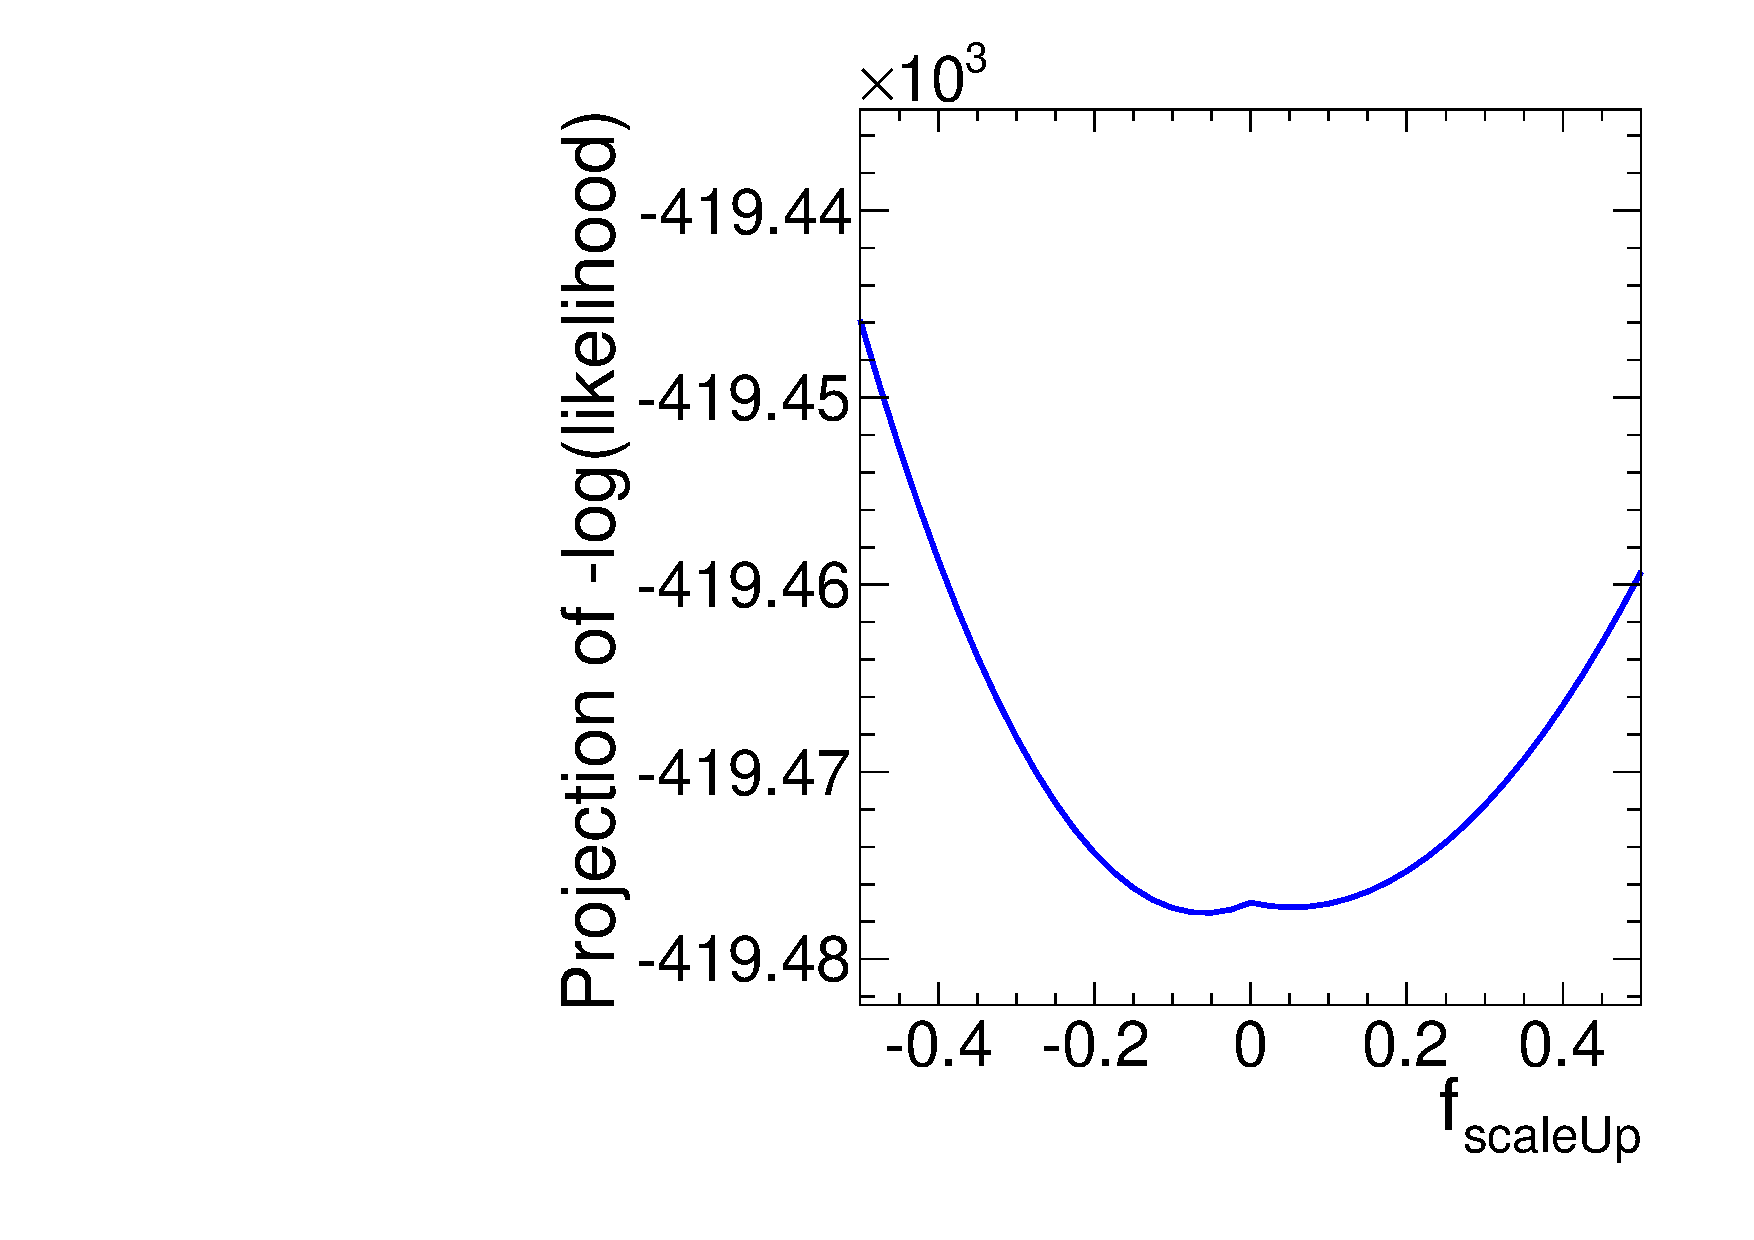
\includegraphics[width=0.48\textwidth]{figs/DibosonNLLfSU.pdf}
%    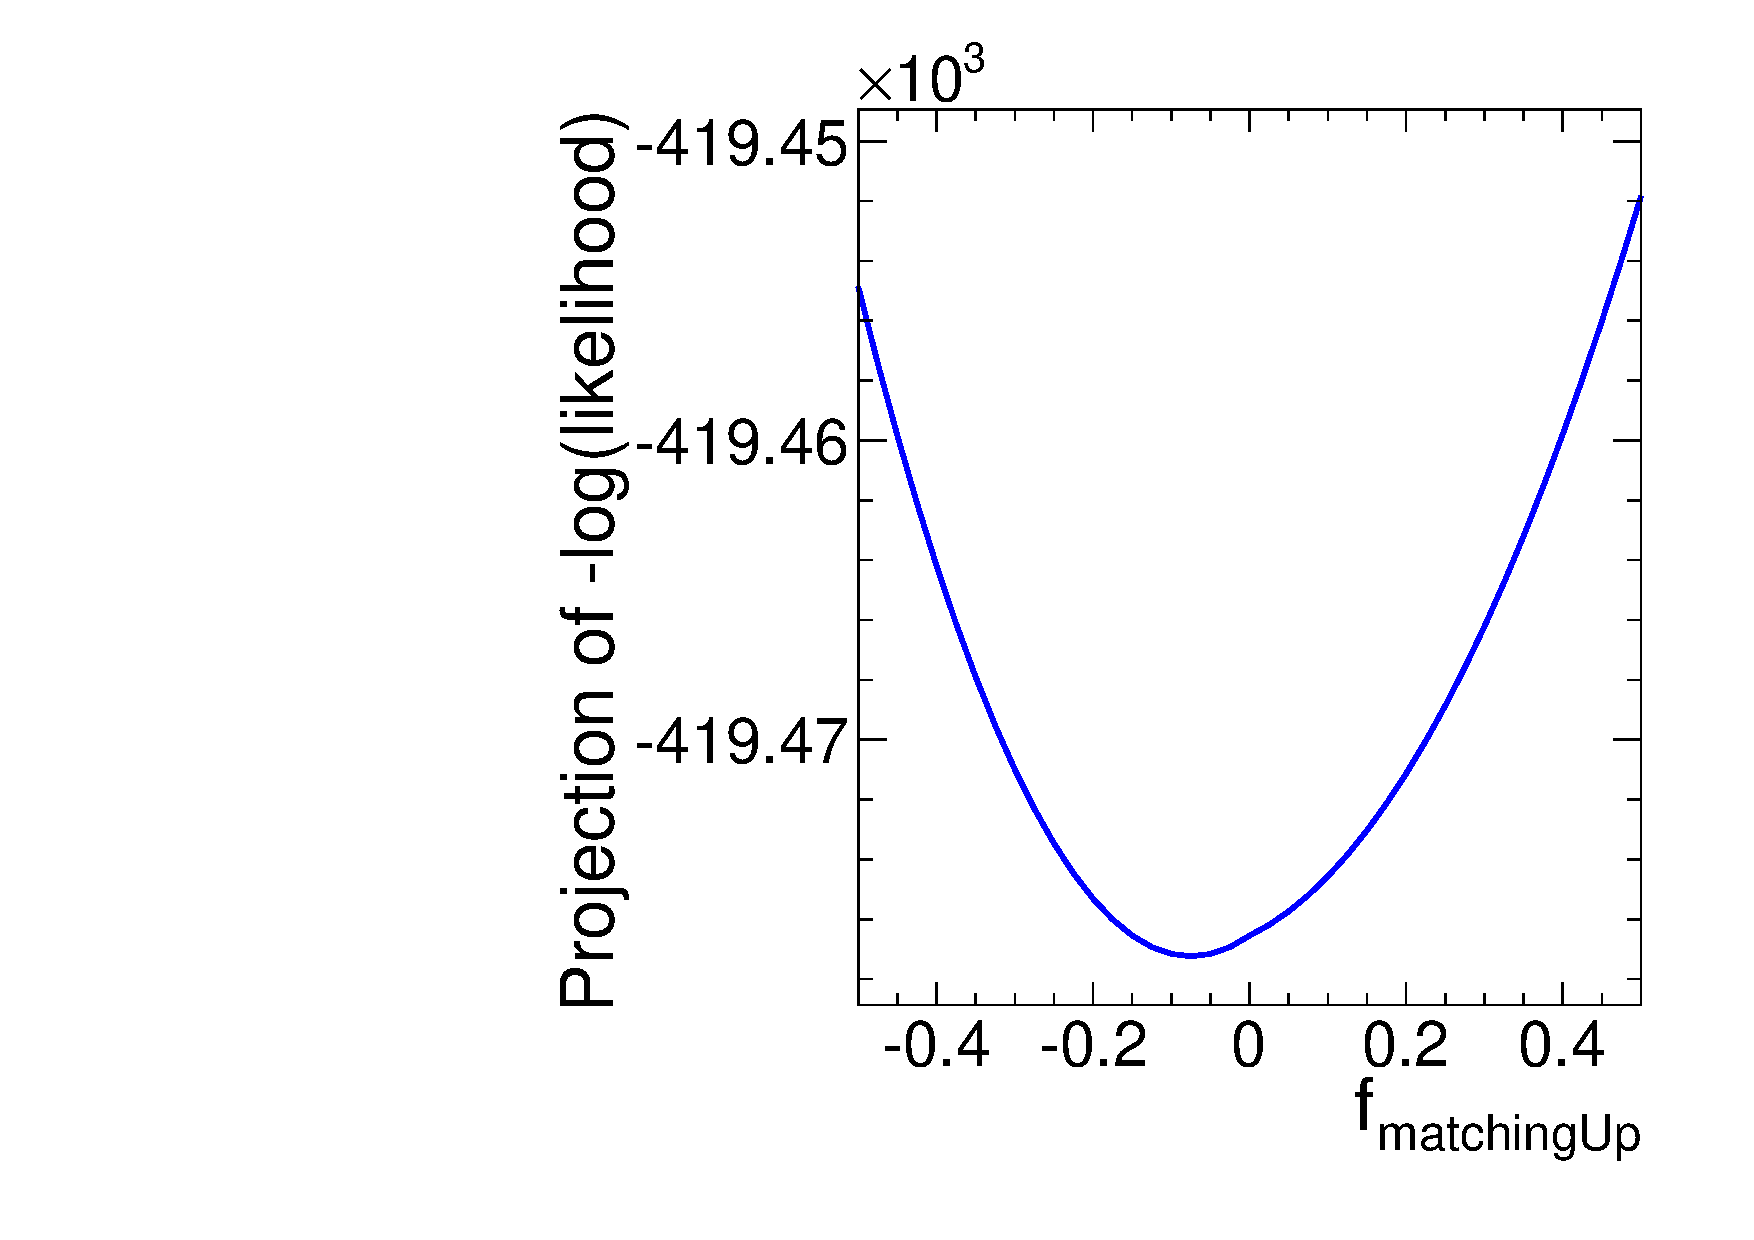
\includegraphics[width=0.48\textwidth]{figs/DibosonNLLfMU.pdf}
%    \caption{The scan of the negative log likelihood for the 
%factrization/renormalization and ME-PS matching scales. They have the 
%usual parabolic distribution with minimum near 0. The minimum values 
%correspond to the ones obtained in our nominal fit and listed in 
%Table~\ref{tab:wjetsscale}. }
%    \label{fig:q2NLLscan}}
%\end{figure}
%%%%%%%%%%%%%



%%%%%%%%%%%%%%%%%%%%%%%%%%%%%%%%%%%%%%%%%%%%
\subsection{Jet Energy Scale: AK5 Jets}
\label{sec:topw}
A dedicated analysis of 2010 data by the JetMET group showed that the jet energy
uncertainty for a generic particle-flow jet is within 3\% and the jet resolution
(JER) uncertainty is within 10\%.  For more details, see
Refs.~\cite{jetsyst,jetsyst2}.  The systematic uncertainties in the
JES and JER can affect our signal acceptance and the $m_{jj}$ distribution.
Figure~\ref{fig:ECComparison} shows a comparison of W+jets shape 
obtained using default jet energy scale with those obtained by using 
$\pm 1\sigma$ variation in the default scale.
In the present analysis, we performed several studies to cross check 
and constrain the JES/JER uncertainties. Two such studies are described 
below. We determine that the average uncertainty in the JES for the 
jet kinematics relevant to the present analysis is at the level below 1\% 
and uncertainty in JER is at the level of 10\%. These are in agreement 
with Refs.~\cite{jetsyst,jetsyst2} for jets of $p_T > 35$~\gev and 
$|\eta|<2.4$. The effect of propagating these uncertainties to the 
signal acceptance and diboson yields is minuscule. 
%%%%%%%%%%%%
%%%%%%%%%%%%
\begin{figure}[h!] {\centering
    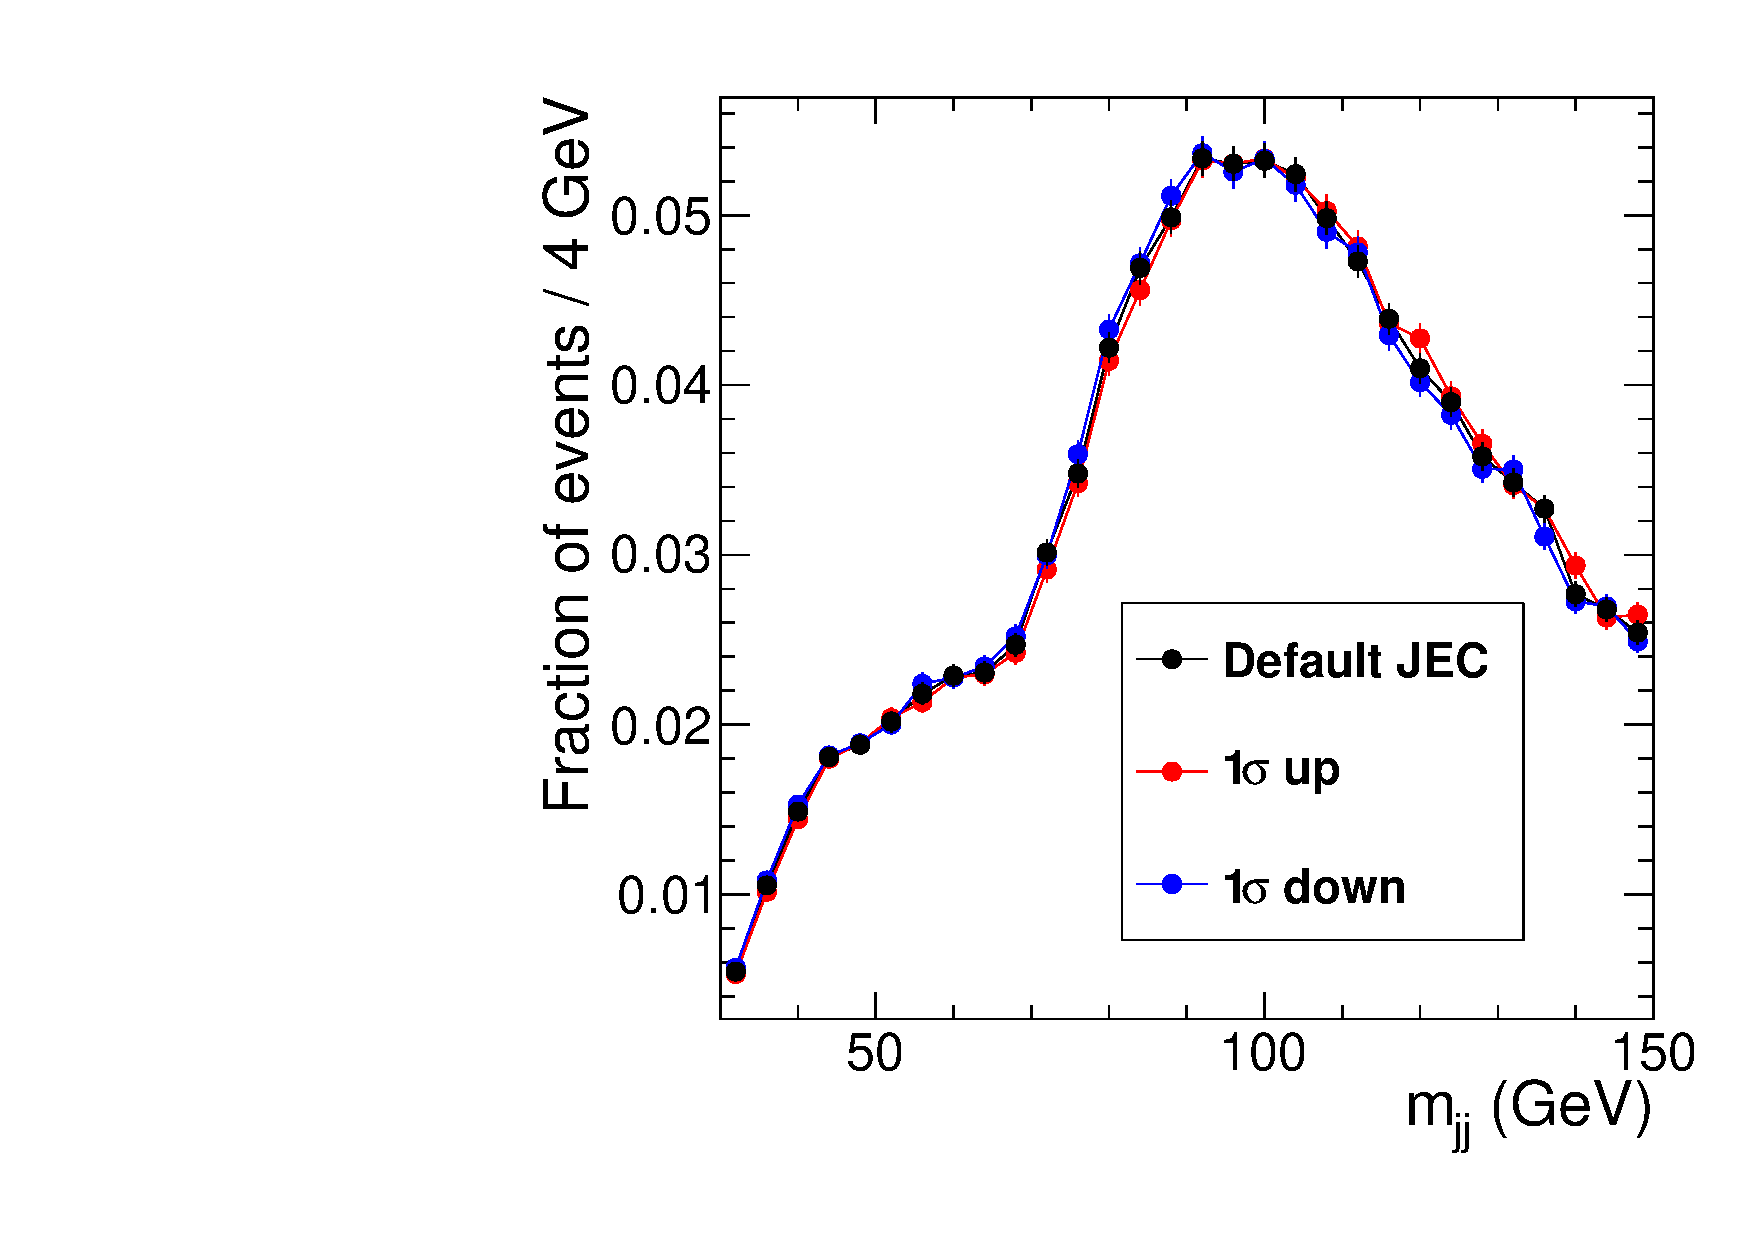
\includegraphics[width=0.5\textwidth]{figs/JECComparison.pdf}
    \caption{Comparison of W+jets shape using default JES and 
    using $\pm 1\sigma$ variation in JES. The selection used here 
    is the same as used for muon no b-tag data.}
    \label{fig:ECComparison}}
\end{figure}
%%%%%%%%%%%%
%%%%%%%%%%%%
%%%%%%%%%%%%
%\subsubsection{Scan of jet energy scale}
%In this study we scan the JES from -5\% to +5\% and repeat the fit. 
%We performed  this test in a subset of the muon data. 
%The $\chi^2$ of the fit is plotted in
%Figure~\ref{fig:JESScanchi2} as a function of the JES shift. 
%
%The minimum in $\chi^2$ is consistent
%with the value obtained from hadronic W candidates in top
%quark events (described below) and the fit has a stable, well defined minimum. 
%Note that the above study serves a crosscheck.
%%%%%%%%%%%%%
%\begin{figure}[h!] {\centering
%    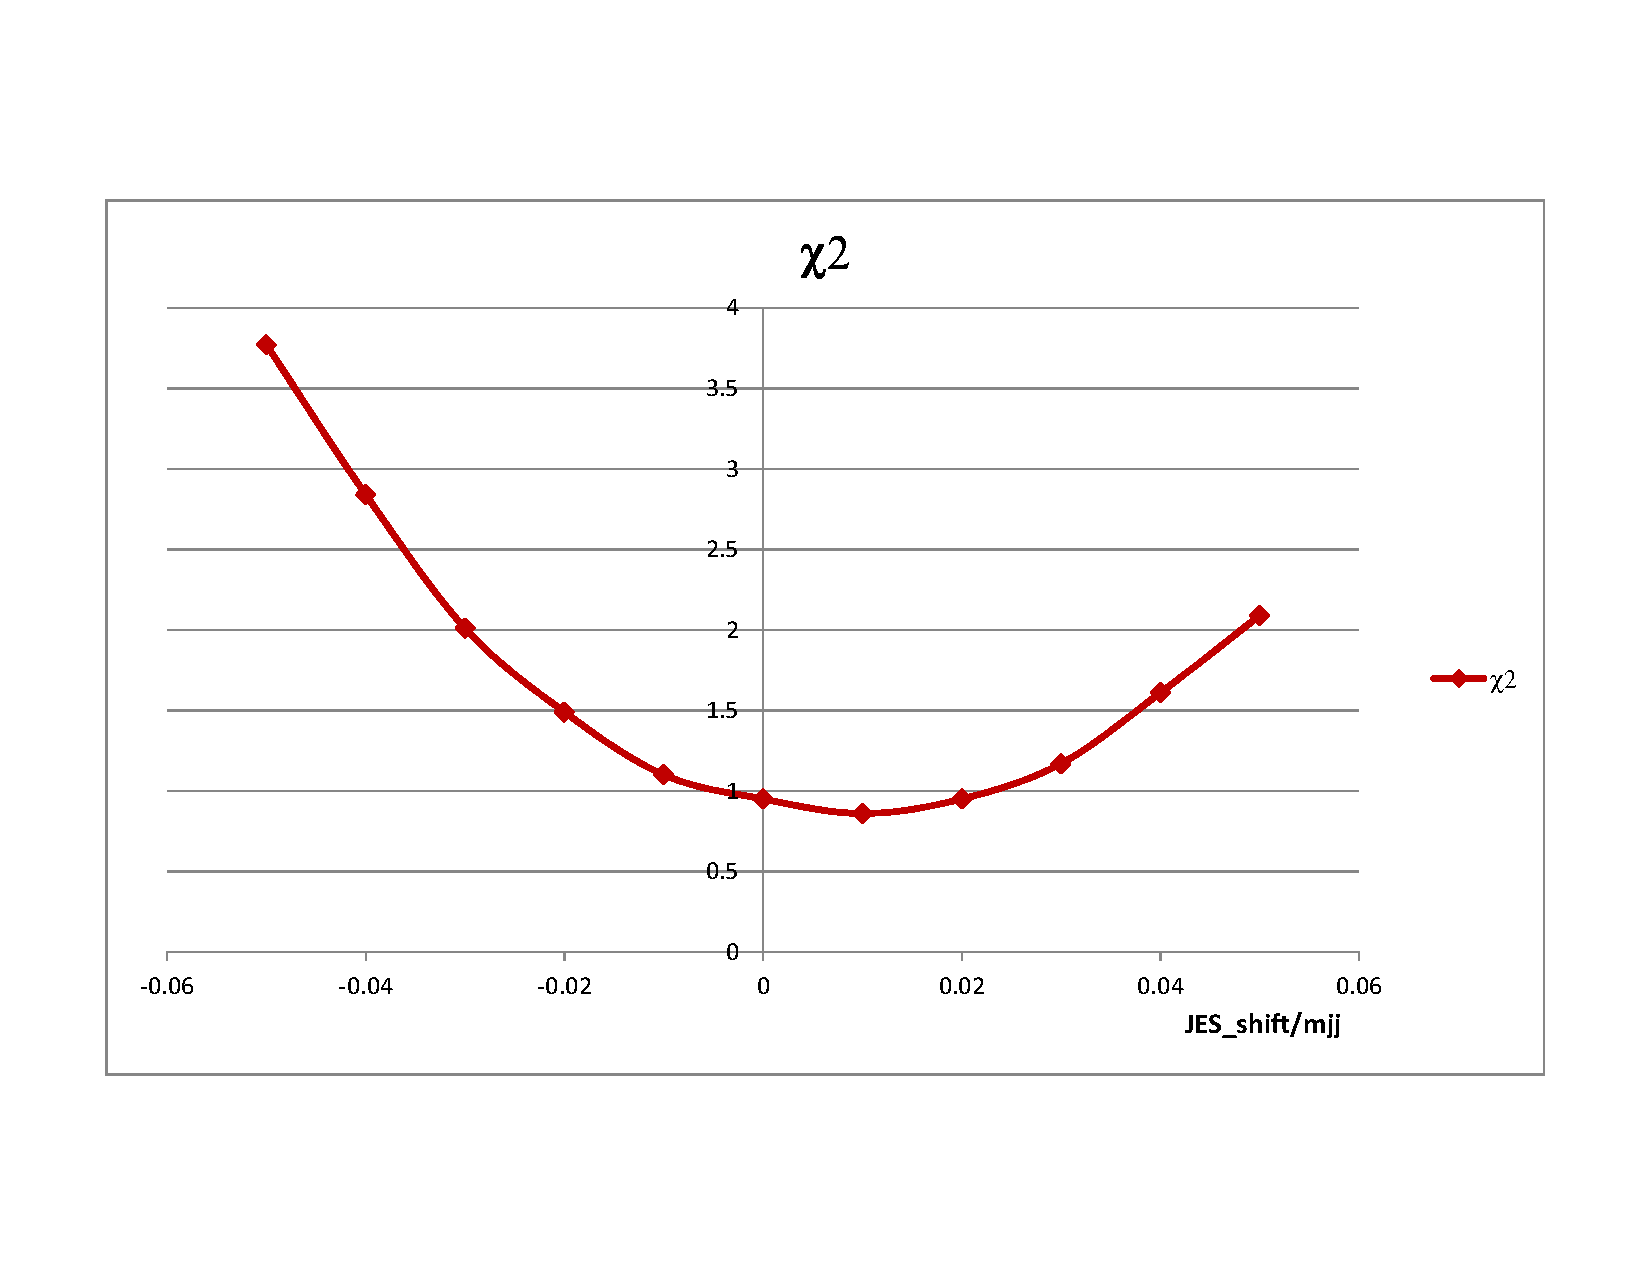
\includegraphics[width=0.5\textwidth]{figs/JES_scan.pdf}
%    \caption{$\chi^2$ of the fit vs JES shift for muon no b-tag data.}
%    \label{fig:JESScanchi2}}
%\end{figure}
%%%%%%%%%%%%

%%%%%%%%%%%%%%%%%%%%%%%%%%%%%
\subsection{Resolved Jets Control Region: $t\bar{t}$}
\label{sec:ttbar_resulved}

At LHC the top pair production rate is fairly large, almost four times larger than the diboson production
rate. According to the Standard Model, the top quark decays into $W$
boson and $b$ quark with branching fraction of about 100\%. When we
select events in which one $W$ boson decays leptonically
(\textit{i.e.}, $W\to e\nu, \mu\nu$) and the other $W$ boson decays
into quark pairs thus leading to a semileptonic final state, then the
signal purity is very high.  The final state consists of a high energy
lepton, large missing $E_T$, and four jets of which two are
$b$-tagged. The hadronic W candidates are formed from two anti-btagged
jets.  The invariant mass of the hadronic W candidates (in the muon channel) is shown in
Fig.~\ref{fig:topw:mu_MC}. As an alternative, we convolve the MC templates with a Gaussian resolution function and
repeat the fit on the control sample data (Fig.~\ref{fig:topw:mu_ConvolvedMC}). The Gaussian parameters returned by the fit are $\mu=4.28\pm 0.50$, $\sigma=3.23\pm 0.49$~GeV. They are subsequently used for convolved template fit studies presented in section~\ref{sec:convolvedMCfit}. However, the $W$ mass resolution is dominated by the resolution of the 
jet energy measurement, with JES systematics accounted for as described in section~\ref{sec:topw}.
%%%%%%%%%%%%%%%%%%%%%
%%%%%%%%%%%%%%%%%%%%%
\begin{figure}[htb] 
  {\centering
    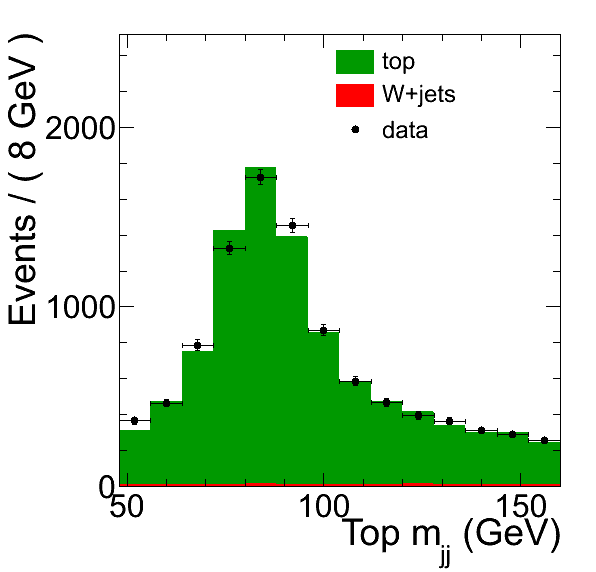
\includegraphics[width=0.49\textwidth]{figs/topwjes/Dibosonlnujj_TopControlSample_muon_Stacked_NoConv.png}
    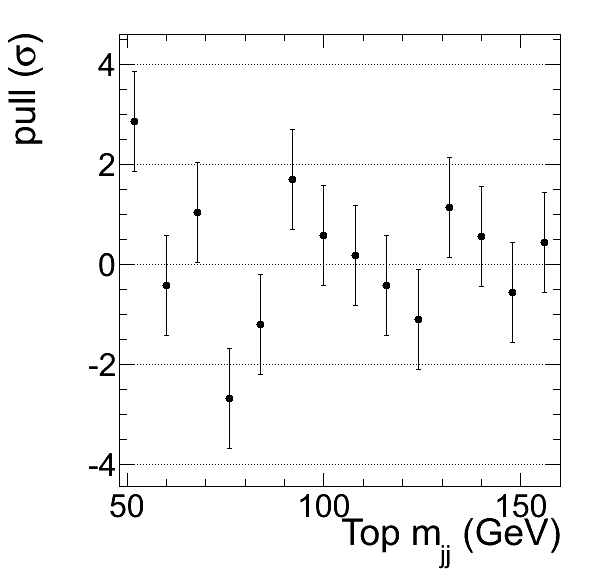
\includegraphics[width=0.49\textwidth]{figs/topwjes/Dibosonlnujj_TopControlSample_muon_Pull_NoConv.png}
    \caption{Template fit to the invariant mass distribution of the hadronic 
      W candidates in the muon semileptonic top sample: stacked backgrounds (left) and normalized residual between data and MC (right).}
    \label{fig:topw:mu_MC}}
\end{figure}
%%%%%%%%%%%%%%
\begin{figure}[htb] 
  {\centering
    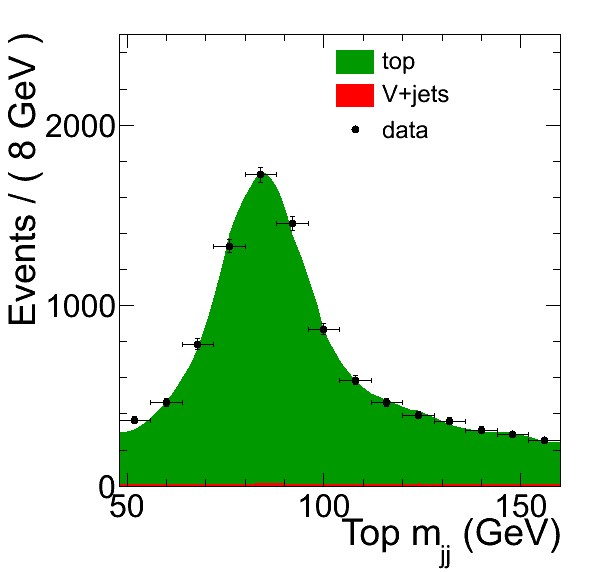
\includegraphics[width=0.49\textwidth]{figs/topwjes/Dibosonlnujj_TopControlSample_muon_Stacked_ConvFit.png}
    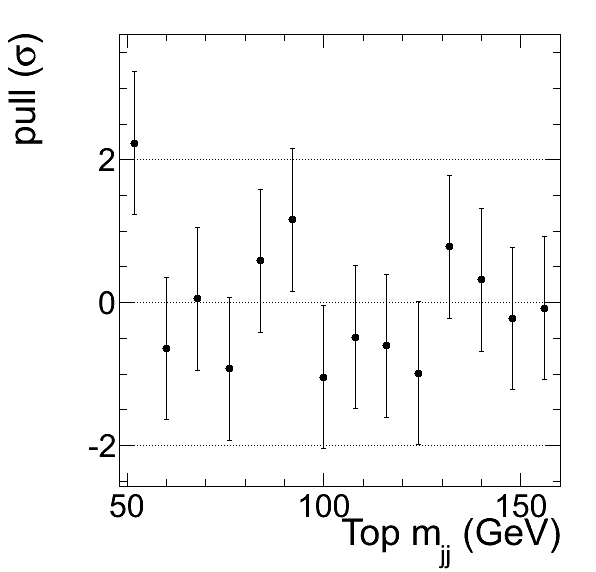
\includegraphics[width=0.49\textwidth]{figs/topwjes/Dibosonlnujj_TopControlSample_muon_Pull_ConvFit.png}
    \caption{Convolved template fit to the invariant mass distribution of the hadronic 
      W candidates in the muon semileptonic top sample: stacked backgrounds (left) and normalized residual between data and MC (right).}
    \label{fig:topw:mu_ConvolvedMC}}
\end{figure}
%%%%%%%%%%%%%%
%%%%%%%%%%%%%%%%%%%%%
\subsubsection{Diboson Mass vs PU}
In addition we study the PileUp dependence of the hadronic W candidate mass in the control sample by fitting it with a Gaussian for low ($NPV<12$), medium ($12<NPV<18$) and high ($NPV>18$) PU scenarios. The results are shown in Fig.~\ref{fig:pu_TopControlSampleGausFit}; the mean and $\sigma$ values are fitted with straight lines with the resultant parameters listed in Table~\ref{tab:pu_TopControlSampleGausFit}. As expected, there is a small increase in the mean \& resolution as a function of PU, while the discrepancies between data and MC remain constant.
%%%%%%%%%%%%%%
\begin{figure}[htb] 
  {\centering
    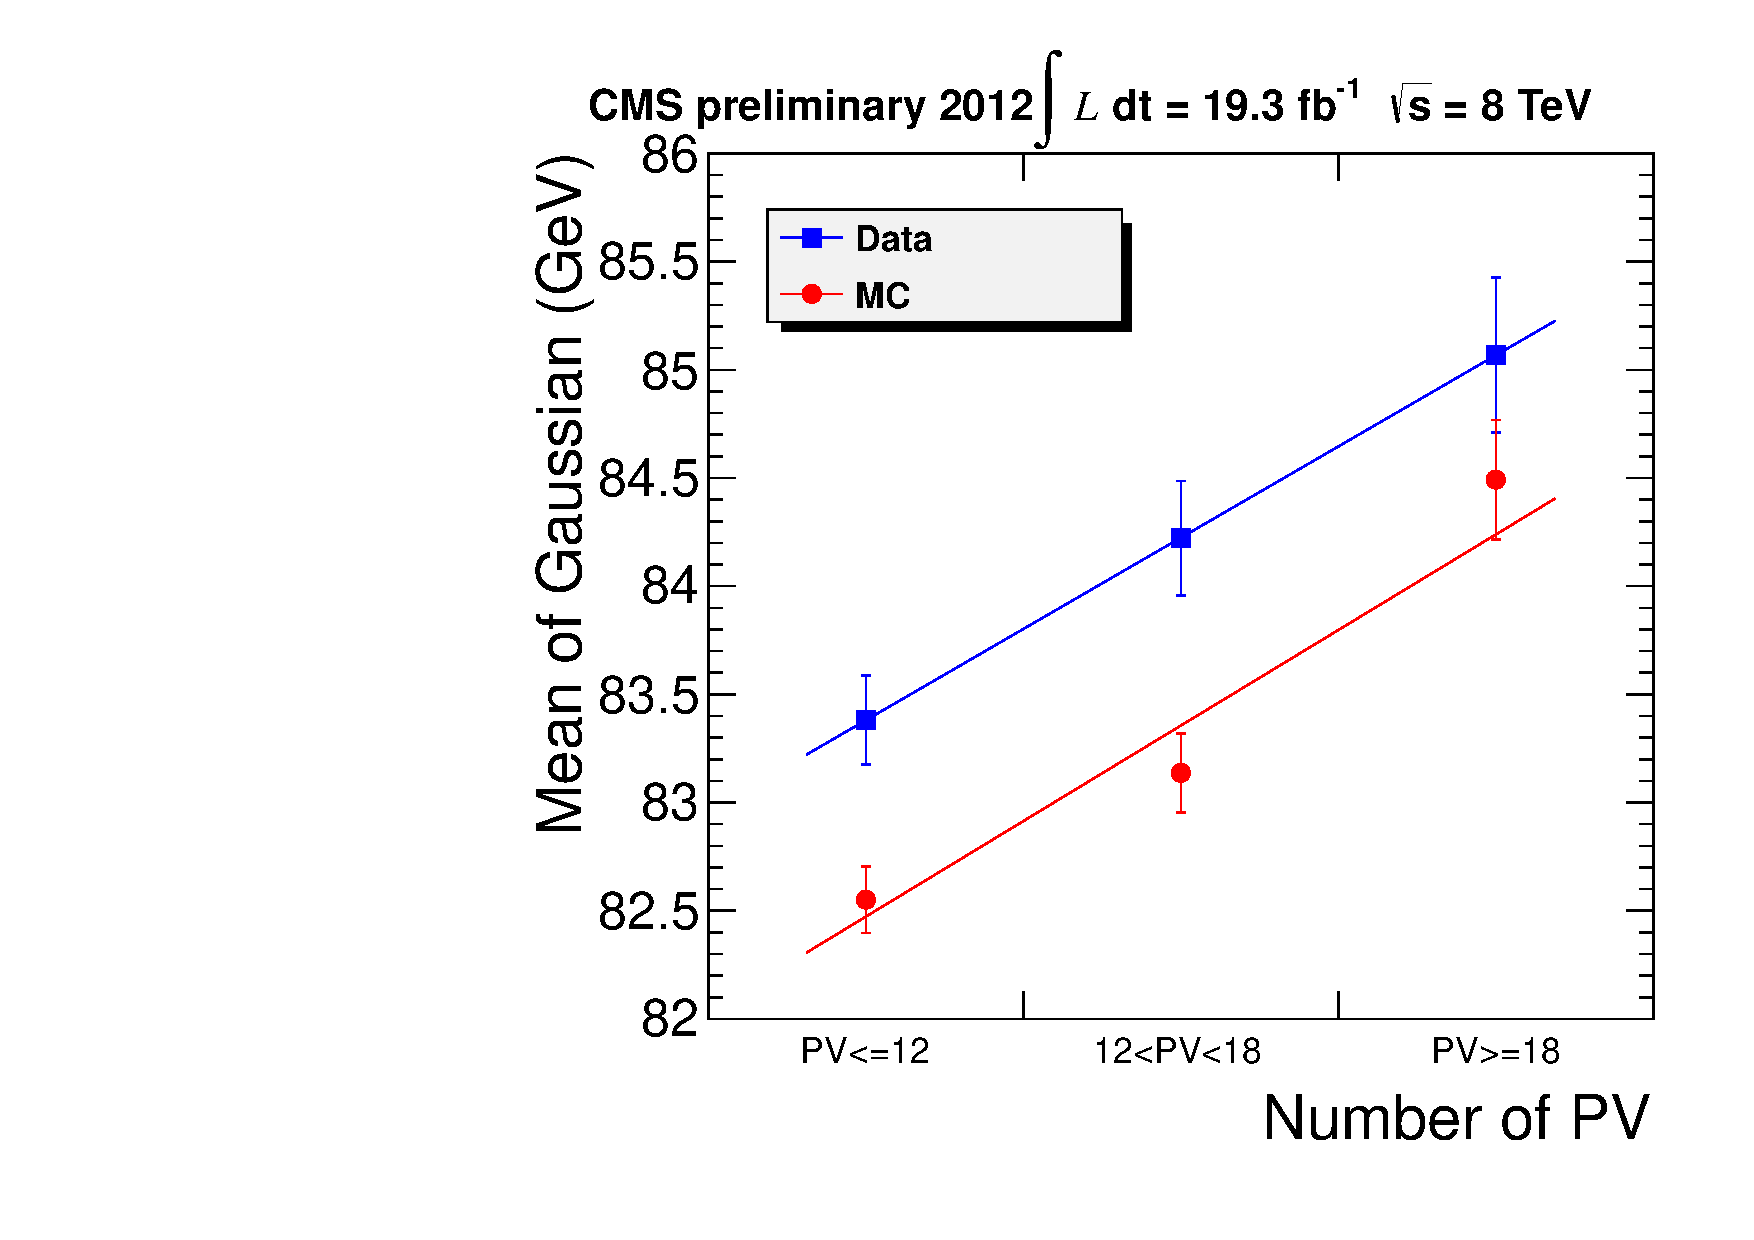
\includegraphics[width=0.49\textwidth]{figs/puchecks/DibosonMassVsPU_mean.pdf}
    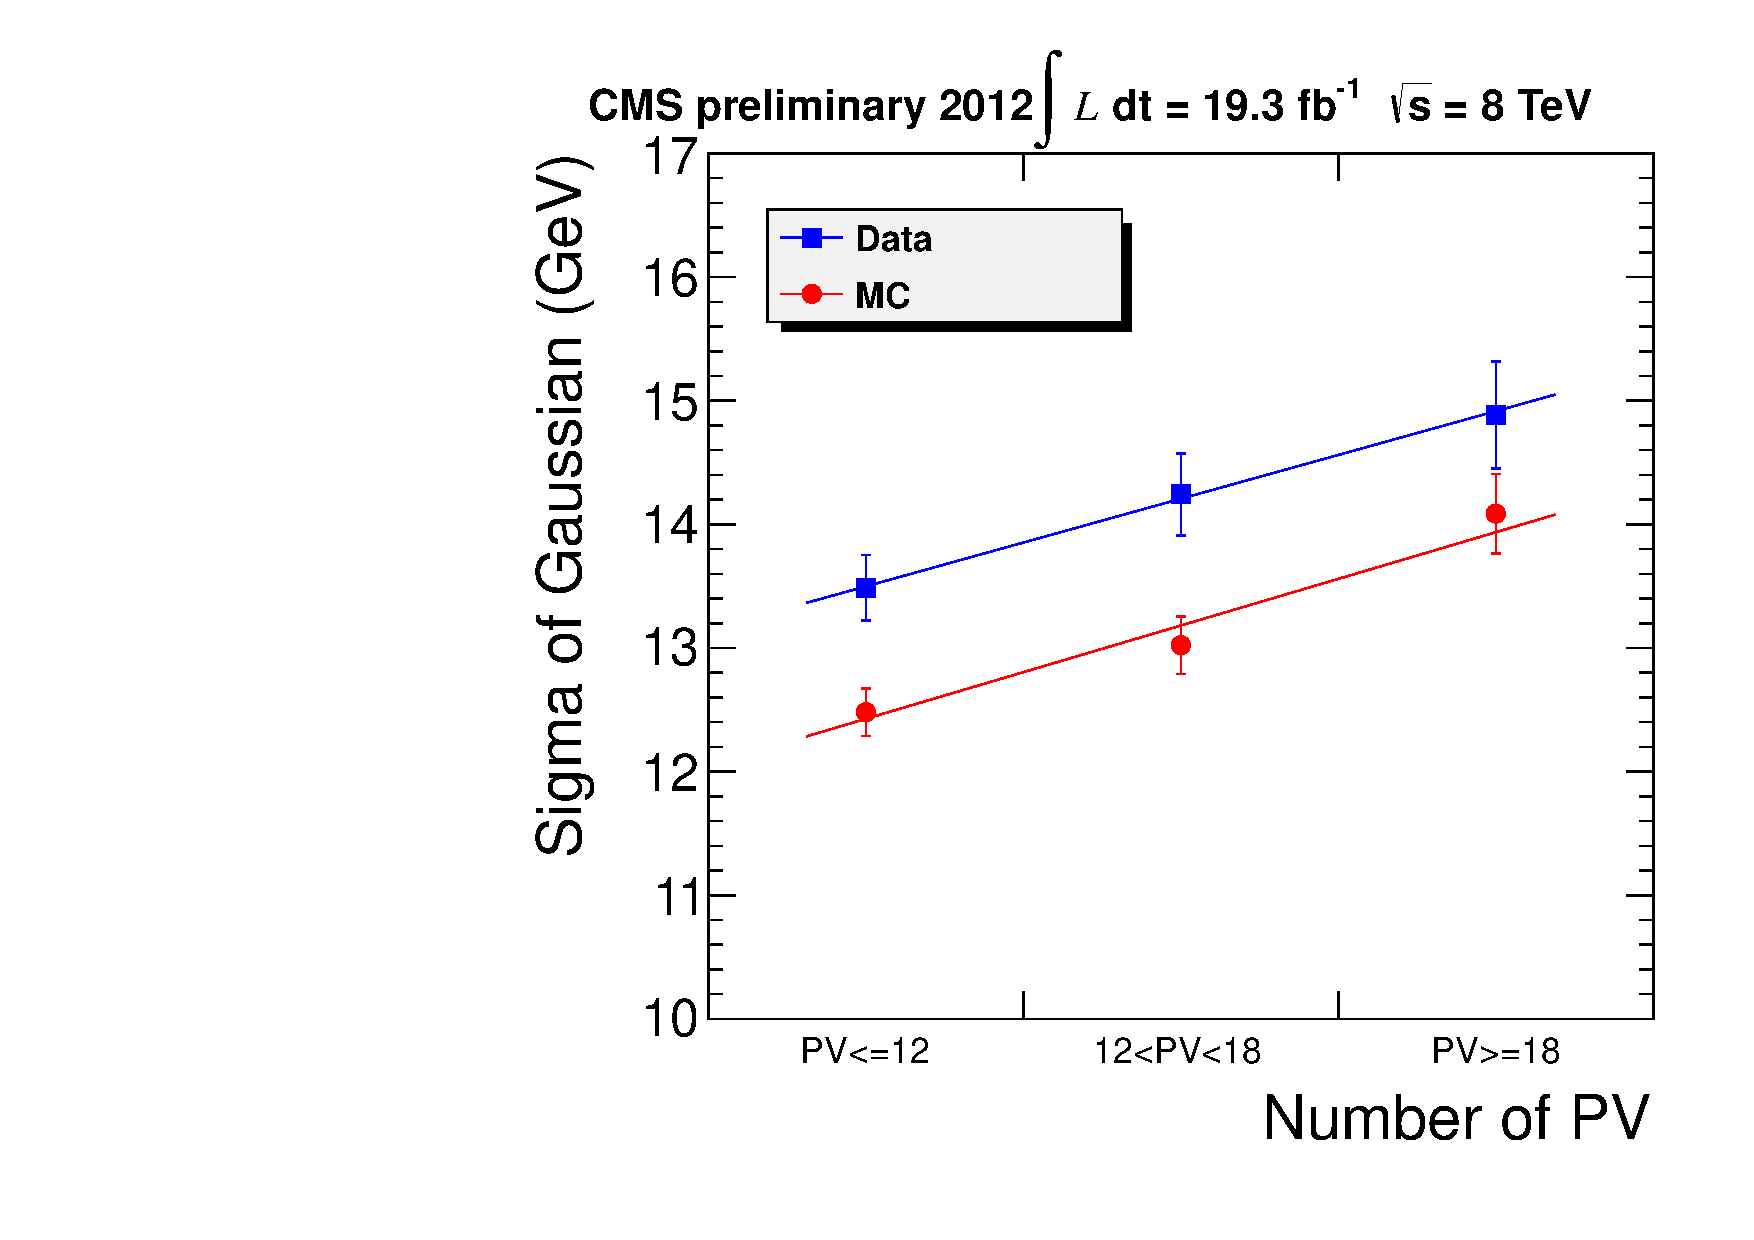
\includegraphics[width=0.49\textwidth]{figs/puchecks/DibosonMassVsPU_sigma.pdf}
    \caption{Gaussian fit results to the invariant mass distribution of the hadronic 
      W candidates in the muon semileptonic top sample for low ($NPV<12$), medium ($12<NPV<18$) and high ($NPV>18$) PU scenarios: mean (left) and $\sigma$ (right).}
    \label{fig:pu_TopControlSampleGausFit}}
\end{figure}
%%%%%%%%%%%%%%
%%%%%%%%%%%%%%%%%%%%%%%%%%
 \begin{table}[h!]
   \begin{center}
   \begin{tabular}{l|cc}
  \hline
  parameter & constant & slope \\
  \hline                                  
  $\mu_{MC}$                                  & $82.0\pm 0.2$ & $0.09\pm 0.01$ \\
  $\mu_{Data}$                                  & $83.0\pm 0.3$ & $0.08\pm0.02$ \\
  $\sigma_{MC}$                               & $12.0\pm 0.3$ & $0.08\pm 0.02$ \\
  $\sigma_{Data}$                               & $13.1\pm 0.3$ & $0.07\pm 0.02$ \\
  \hline
   \end{tabular}
   \end{center}
   \caption{Linear dependence of the mean and resolution of the gaussian fit to the invariant mass distribution of the hadronic 
      W candidates in the muon semileptonic top sample. The increase as a function of $NPV$ is statistically consistent between MC and Data.} 
   \label{tab:pu_TopControlSampleGausFit}
 \end{table}
%%%%%%%%%%%%%%%%%%%%%%%%%

%%%%%%%%%%%%%%%%%%%%%%%%%%%%%
%--------------------------------------------------
\subsection{Jet Energy Scale: CA8 Jets}
\label{sec:systematicsCA8}
The CA8 jets are corrected using the AK7 dedicated corrections.  
The systematic uncertainty is estimated by varying up and down the jet energy uncertainties and computing the effect on the mean jet mass in the 
$t\bar{t}$ control sample.  

Additional uncertainties are added in quadrature to the AK7 jet uncertainties in order to account for the CA8 jets.  
In order to compute this additional uncertainty, we take signal MC samples and match AK7 jets to CA8 jets and 
take the fractional difference between them as an additional uncertainty. 
The matching is done for AK7 and CA8 collections for events passing preselection criteria and are matched with $\Delta R < 0.3$ criteria.
The fractional difference is computed as a function of $p_T$ and $\eta$ and is fit with a Gaussian.
In the top left and right of Fig.~\ref{fig:CA8vAK7}, we show the fitted mean and sigma fractional difference between the matched AK7 and CA8 jets 
as a function of jet $\eta$.
In the bottom left and right of Fig.~\ref{fig:CA8vAK7}, we show the fitted mean and sigma fractional difference between the matched AK7 and CA8 jets 
as a function of jet $p_T$.

\begin{figure}[htbp]
\centering
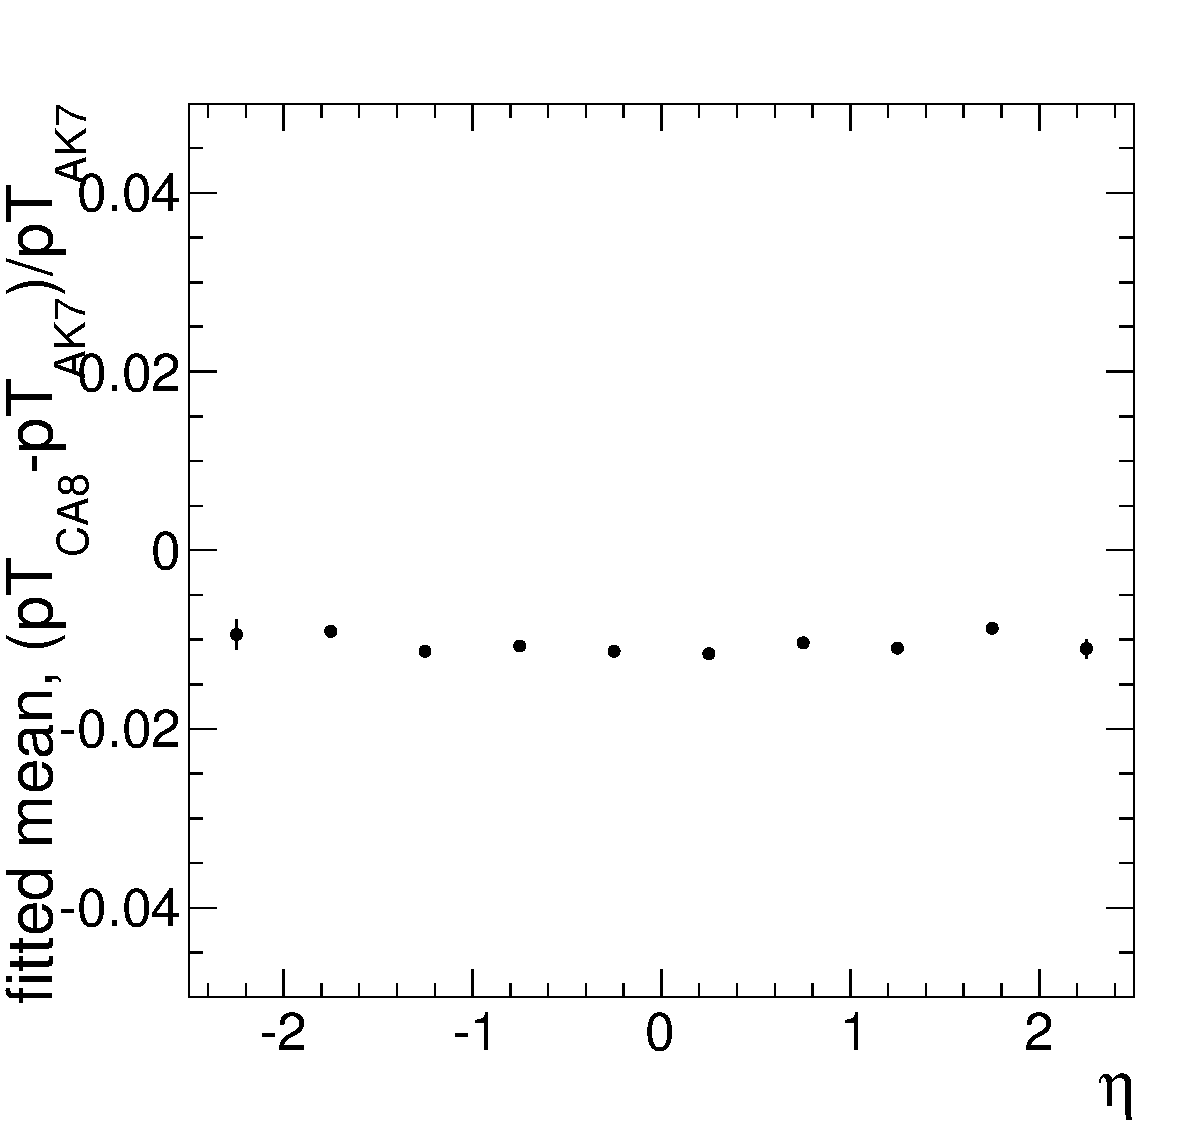
\includegraphics[width=0.48\textwidth]{figs/diff_CA8vAK7_vEta_mean}
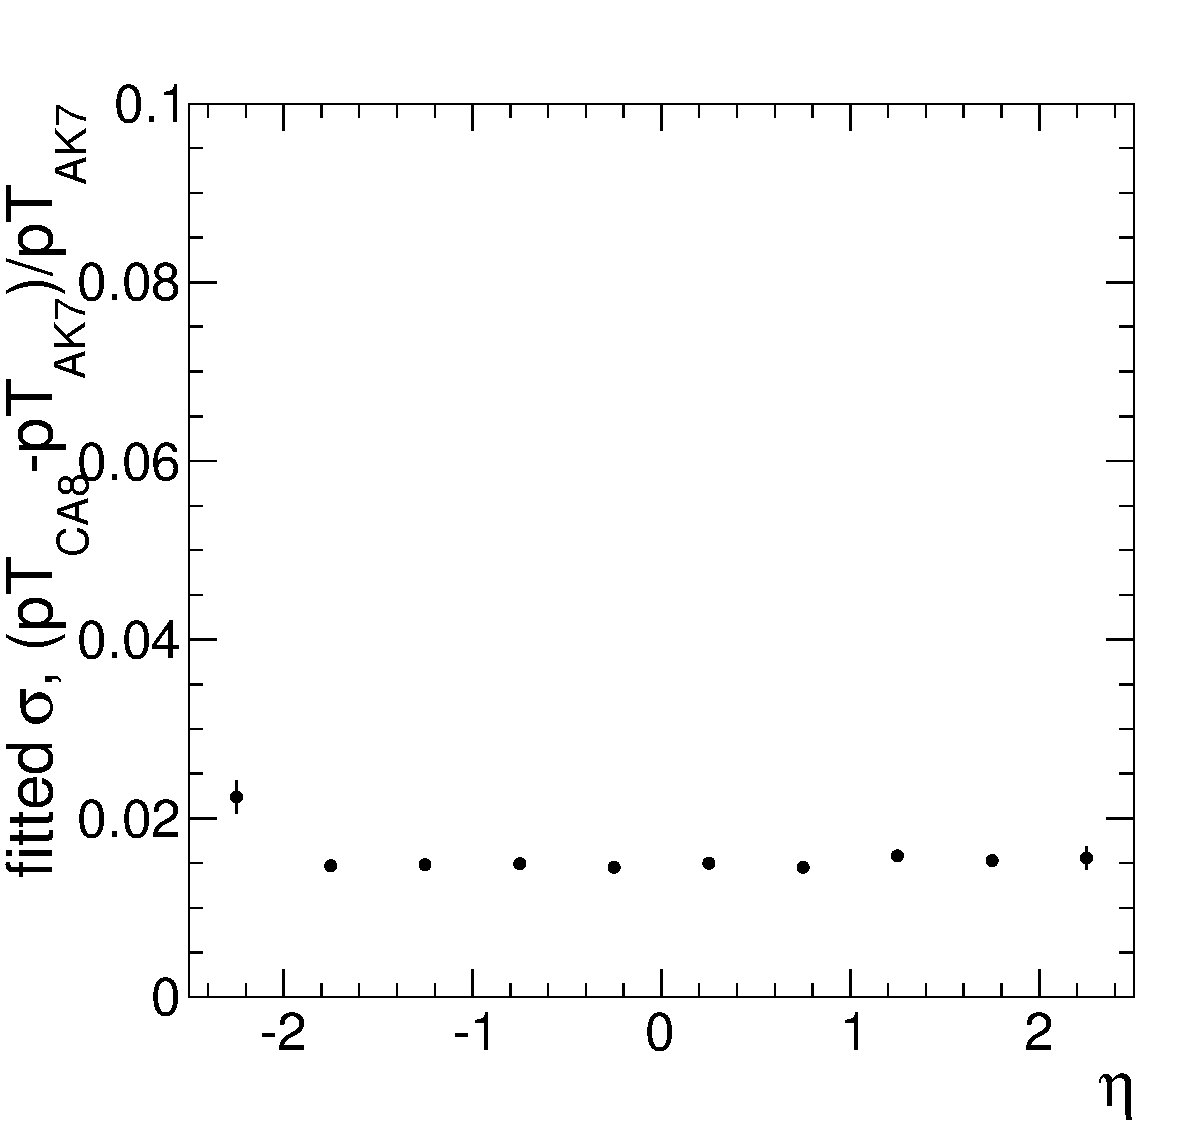
\includegraphics[width=0.48\textwidth]{figs/diff_CA8vAK7_vEta_sigma}\\
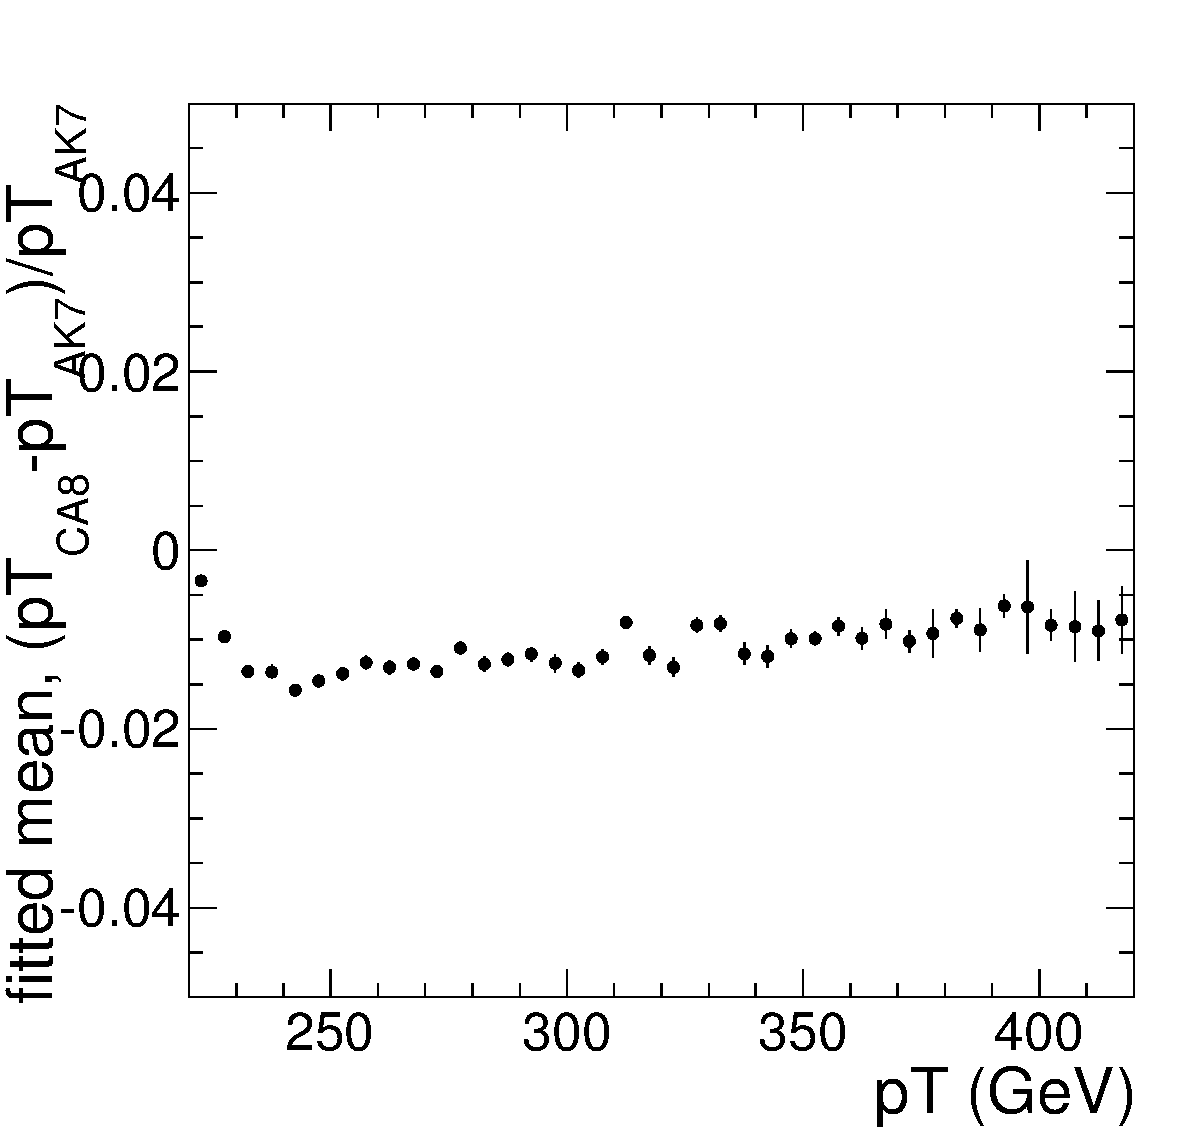
\includegraphics[width=0.48\textwidth]{figs/diff_CA8vAK7_vPt_mean}
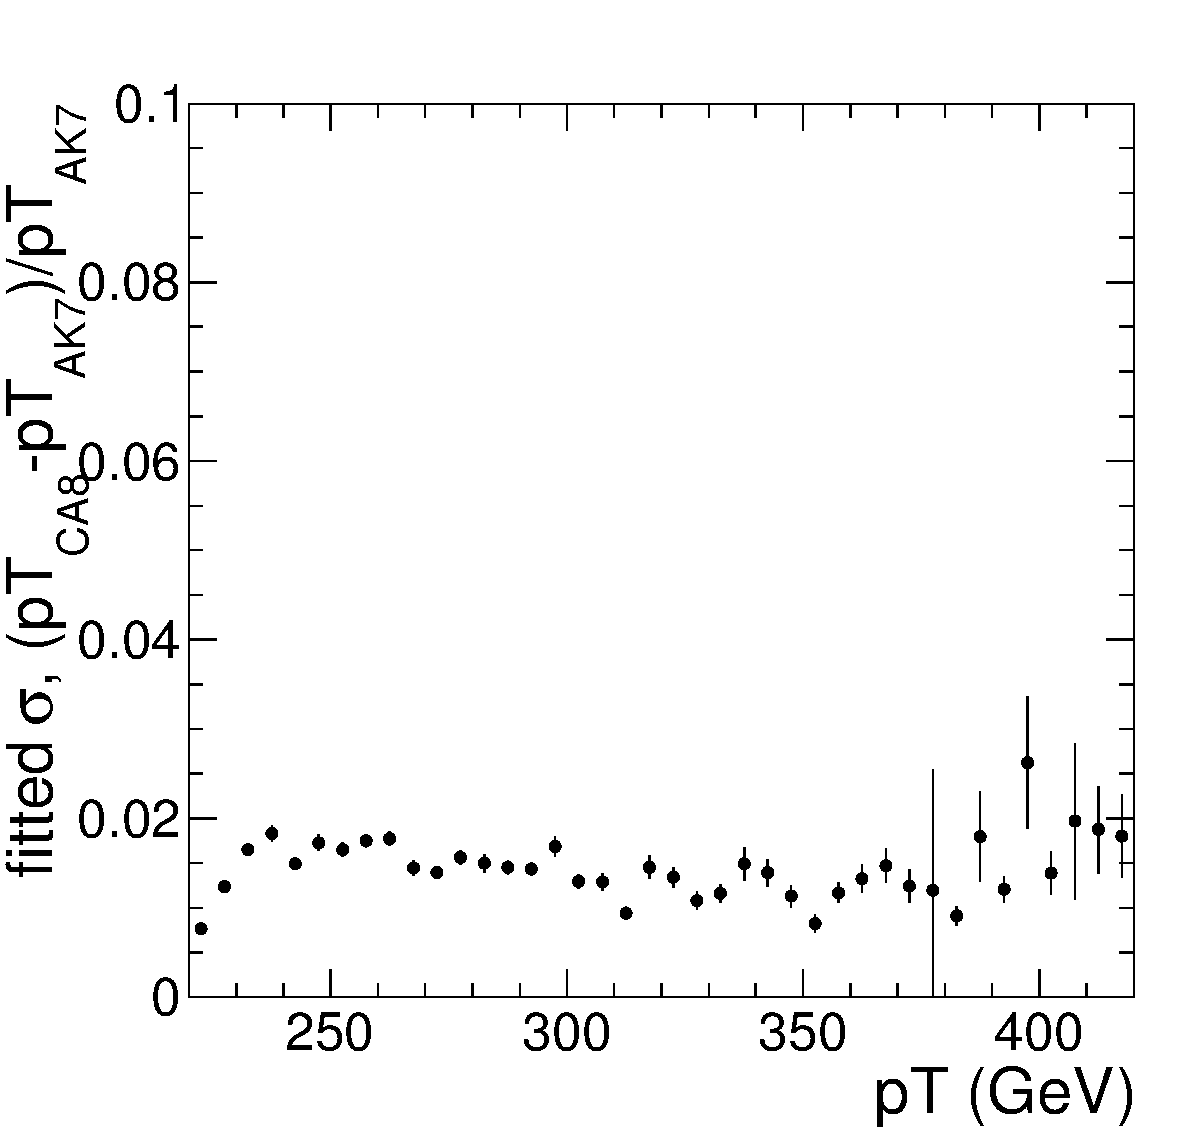
\includegraphics[width=0.48\textwidth]{figs/diff_CA8vAK7_vPt_sigma}\\
\caption{Fitted mean and sigma fractional difference between the matched AK7 and CA8 jet $p_T$ as a function of jet $\eta$ (top) and $p_T$ (bottom).}
\label{fig:CA8vAK7}
\end{figure}

From the plots in Fig.~\ref{fig:CA8vAK7}, we find that an additional 2\% uncertainty on the jet energy scale uncertainty added in quadrature
with the computed AK7 corrections are enough to cover scale differences due to not having dedicated corrections for CA8 jets.

%%%%%%%%%%%%%%%%%%%%%%%%%%%%%
\subsection{Merged Jets Control Region: $t\bar{t}$}
\label{sec:ttbar_merged}

To understand the performance of merged W bosons, we use a control sample of pure W's in the data from the high pT $t\bar{t}$ sample. Namely, we use the standard kinematic preselection cuts described above, but invert the cut on the number of b-tagged AK5 jets outside of the CA8 jet requiring that there is at least one CSV "medium" AK5 b-jet.
To boost statistics, we choose the CA8 jet in the opposite hemisphere of the lepton with the highest mass and a pT $>$ 200 GeV.
This is contrary to the standard selection which uses the high pT CA8 jet in the event with a pT $>$ 200 GeV.

Furthermore, for the $WW/WZ$ and signal contributions, we are concerned with the data/MC scale factor for the {\it pure} W-jet
tagging efficiency.  
In order to understand the part of the $t\bar{t}$ jet mass distribution which contains "real" merged W's and pure combinatorial background
we use the $t\bar{t}$ MC sample. 
By matching the CA8 jet with the hadronic $W$ at generator level in a cone of $\Delta R < 0.3$, we can get expected shapes.  
These plots are shown in Fig.~\ref{fig:genMatchTTbar} before and after a cut on $\tau_2/\tau_1<0.55$.  
The functional forms we choose are $f_{bkg}(x) = {\rm Exp}*{\rm Erf}$ for the unmatched sample and $f_{sig}(x) = {\rm Gaus1} + {\rm Gaus2}$ for the matched sample.

\begin{figure}[htbp]
\centering
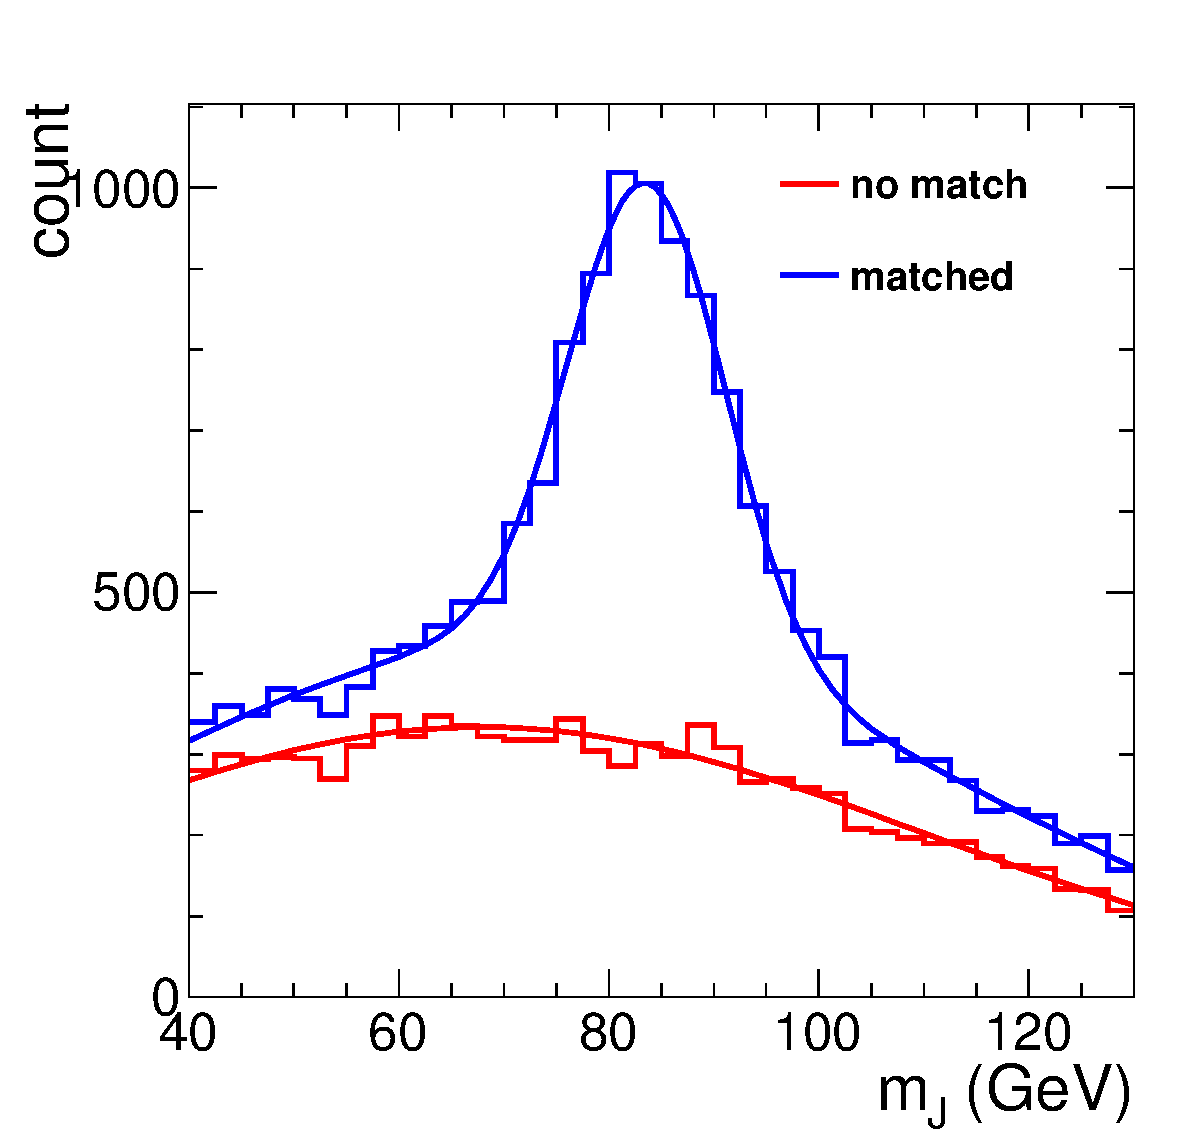
\includegraphics[width=0.48\textwidth]{figs/topwjes/GEN_all_nocut.pdf}
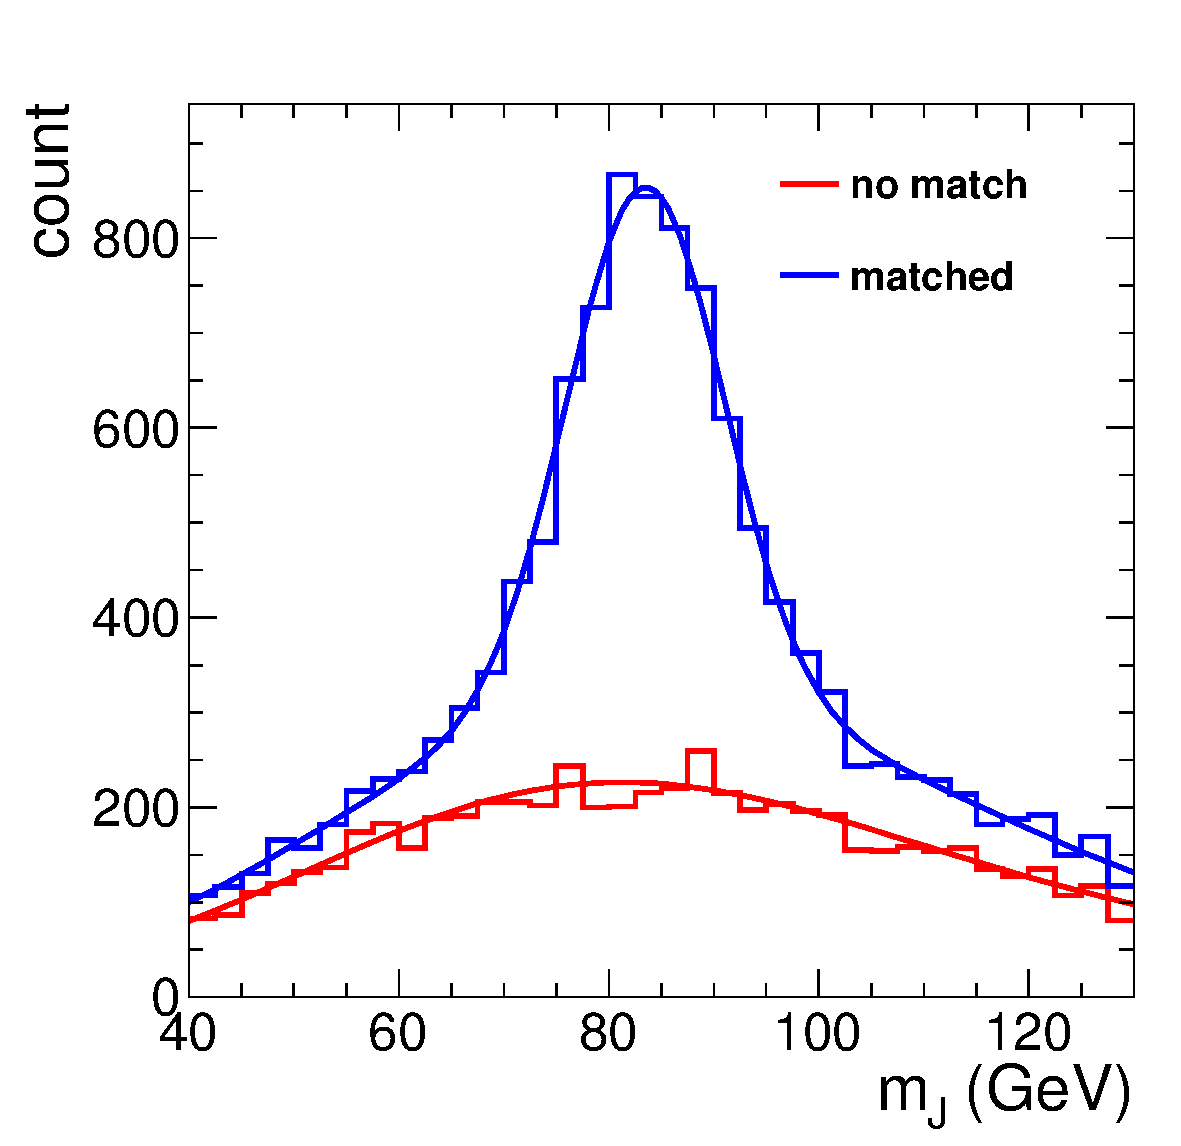
\includegraphics[width=0.48\textwidth]{figs/topwjes/GEN_all_cutT2T1.pdf}
\caption{Matched and unmatched samples of $t\bar{t}$ MC sample in $t\bar{t}$ control region before (left)
and after (right) the cut of $\tau_2/\tau_1<0.55$.}
\label{fig:genMatchTTbar}
\end{figure}

We then extract the scale factors by first estimating the cut efficiency on both data and MC.
This gives us simultaneously "pass" and "fail" samples where we can then simultaneously fit to get the cut efficiency.  
The difference in the data and MC efficiencies are taken as the W-tagging efficiency.
The fit results are shown in Fig.~\ref{fig:ttbarControl_nocut}.
The fitting functions are motivated by the shapes in Fig.~\ref{fig:genMatchTTbar}.
The scale factor for electrons and muons are computed to be 0.997 and 0.993, respectively where the uncertainty on the scale factor is 7.5\%.
These scale factors are applied to the $WW/WZ$ and signal contributions.  

To extract the jet mass scale uncertainty and resolution scale factor, we fit the mass peak in the signal region.  
%The $t\bar{t}$ control sample is fit with a functional form $f(x) = {\rm Exp}*{\rm Erf} + {\rm Gaus1}*{\rm Gaus2}$.
The fits are shown for the medium $W$-tag cut in the right side plots of Fig.~\ref{fig:ttbarControl_nocut}.
The fit means and sigma of the core Gaussian in the muon channel is found to be:
\begin{eqnarray}
\langle m \rangle_{\rm MC} = 83.3 \pm 0.5~{\rm GeV}{\rm {~,~}}\sigma_{\rm MC} = 7.1 \pm 0.3~{\rm GeV} \\
\langle m \rangle_{\rm data} = 83.7 \pm 0.5~{\rm GeV}{\rm {~,~}}\sigma_{\rm MC} = 7.7 \pm 0.4~{\rm GeV} 
\end{eqnarray}

The fit means and sigma of the core Gaussian in the electron channel is found to be:
\begin{eqnarray}
\langle m \rangle_{\rm MC} = 83.3 \pm 0.6~{\rm GeV}{\rm {~,~}}\sigma_{\rm MC} = 6.7 \pm 0.4~{\rm GeV} \\
\langle m \rangle_{\rm data} = 83.9 \pm 0.6~{\rm GeV}{\rm {~,~}}\sigma_{\rm MC} = 7.9 \pm 0.5~{\rm GeV}
\end{eqnarray}
We find that the mass scale systematic is unity to within errors but that the W-jet resolution is larger in the data.
Since we do not expect that the resolution should differ between electron and muon channels, we average the difference as 
$\bar{\sigma}_{MC}$  = 7.0 and $\bar{\sigma}_{data}$  = 7.8. 
We correct the MC resolution by 11\% to correct for the difference in data/MC.

\begin{figure}[htbp]
\centering
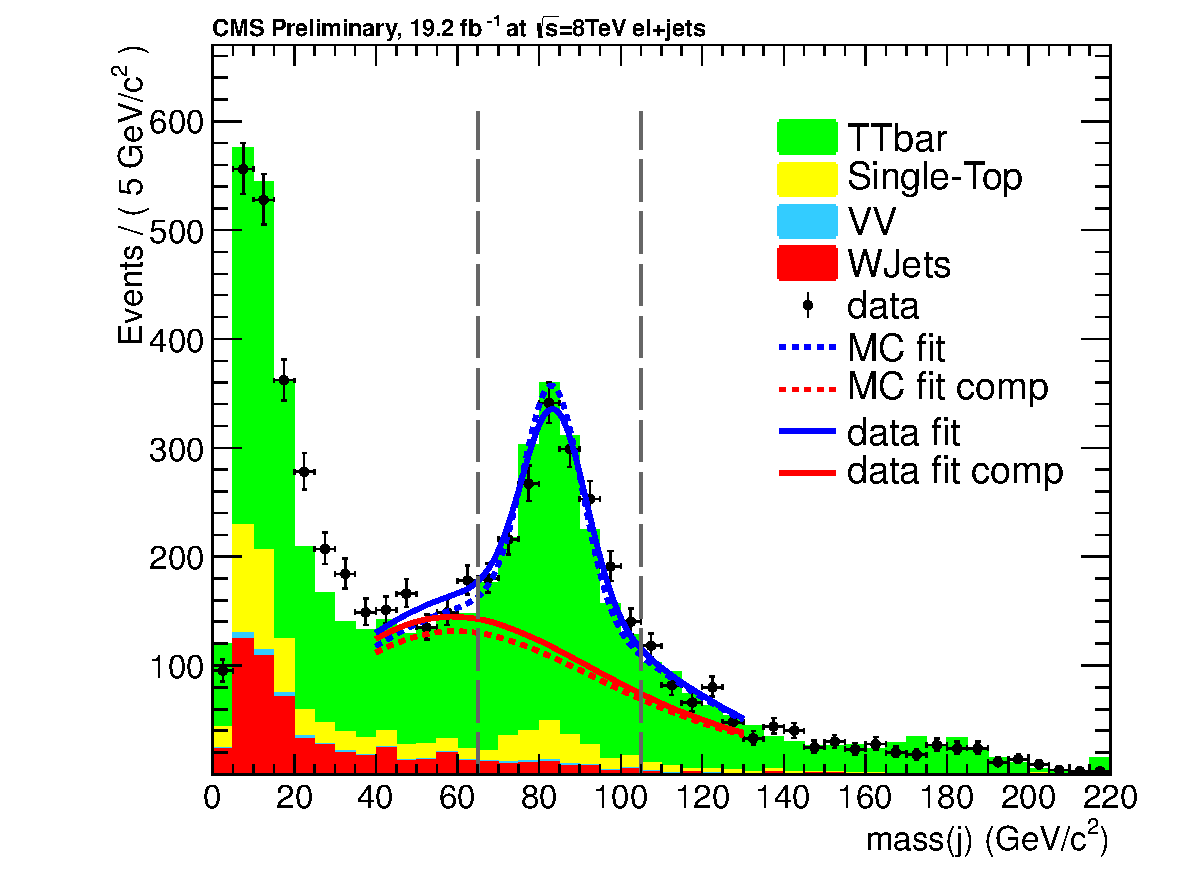
\includegraphics[width=0.45\textwidth]{figs/topwjes/control_medium_el_without_tau2tau1.pdf}
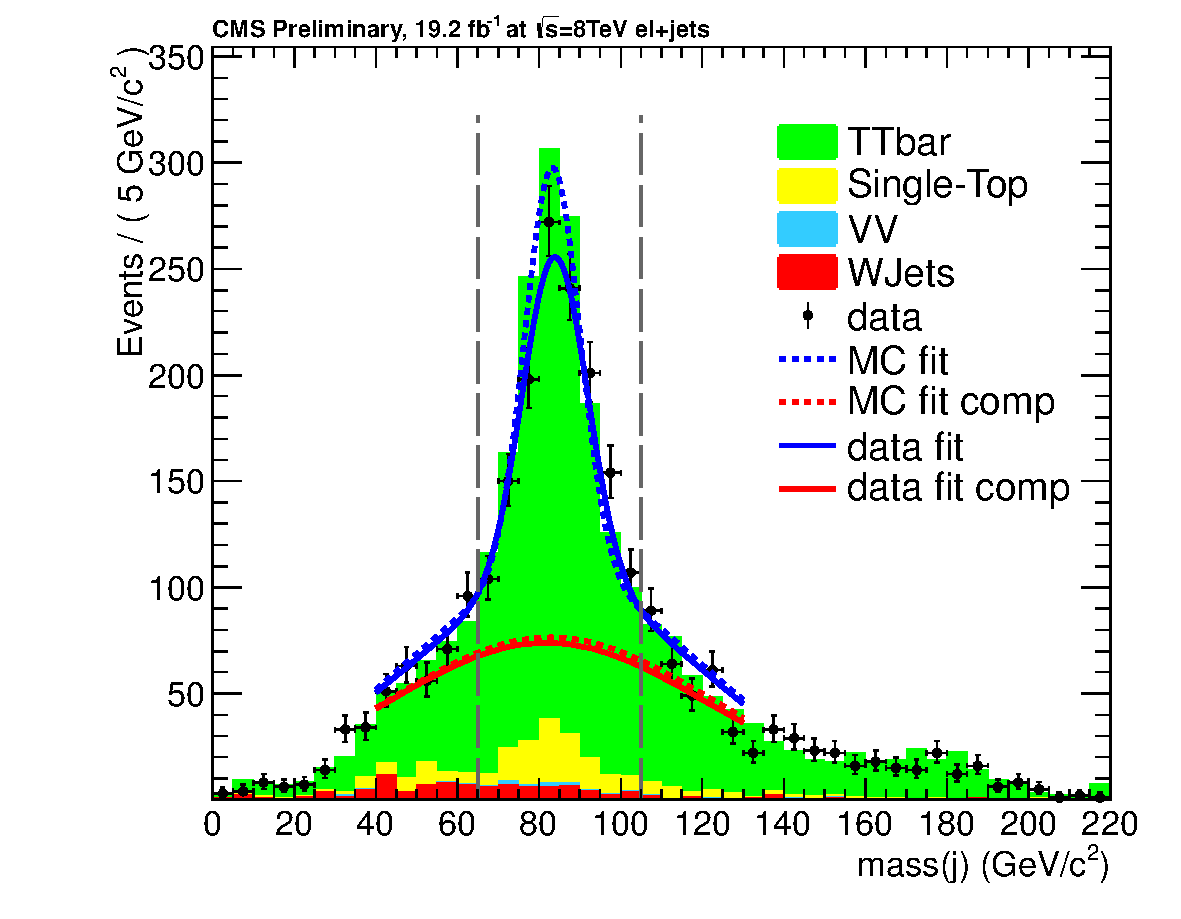
\includegraphics[width=0.45\textwidth]{figs/topwjes/control_medium_el_with_tau2tau1.pdf}\\
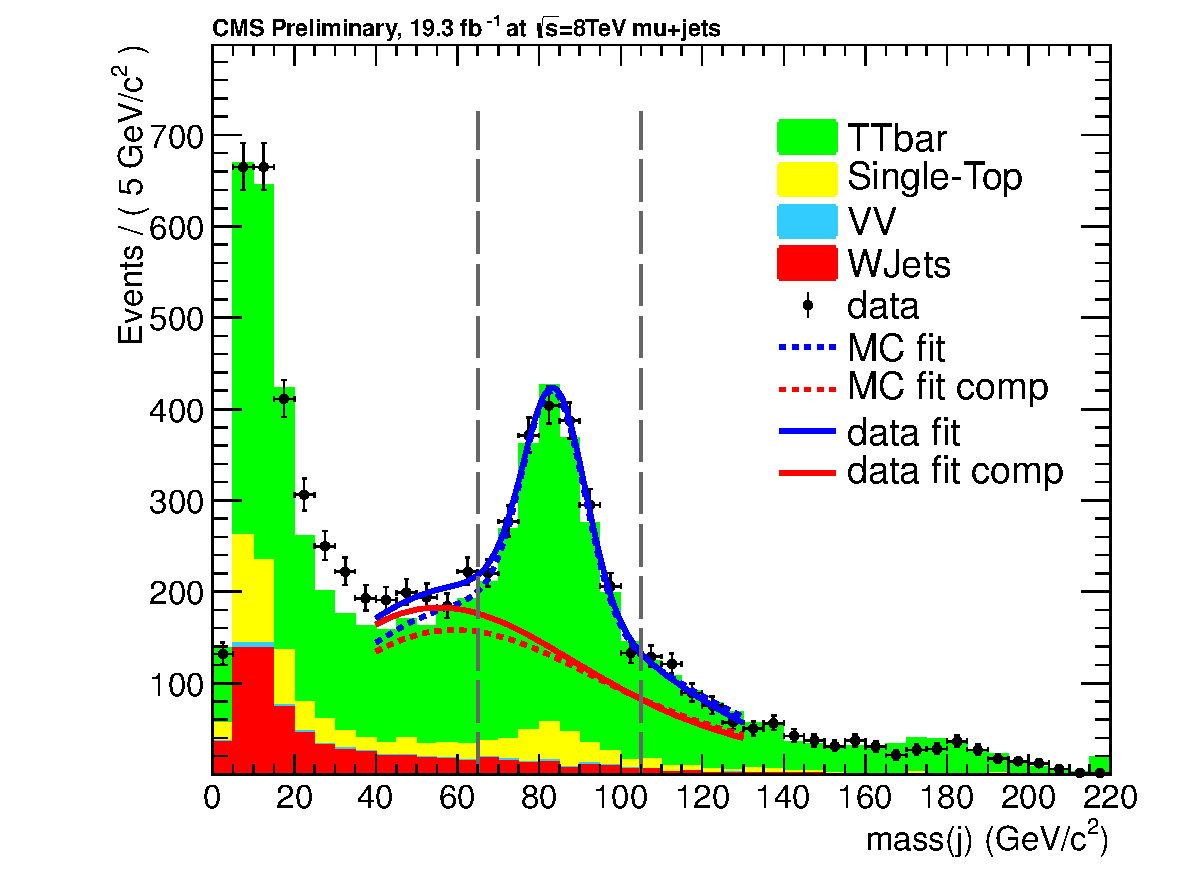
\includegraphics[width=0.45\textwidth]{figs/topwjes/control_medium_mu_without_tau2tau1.pdf}
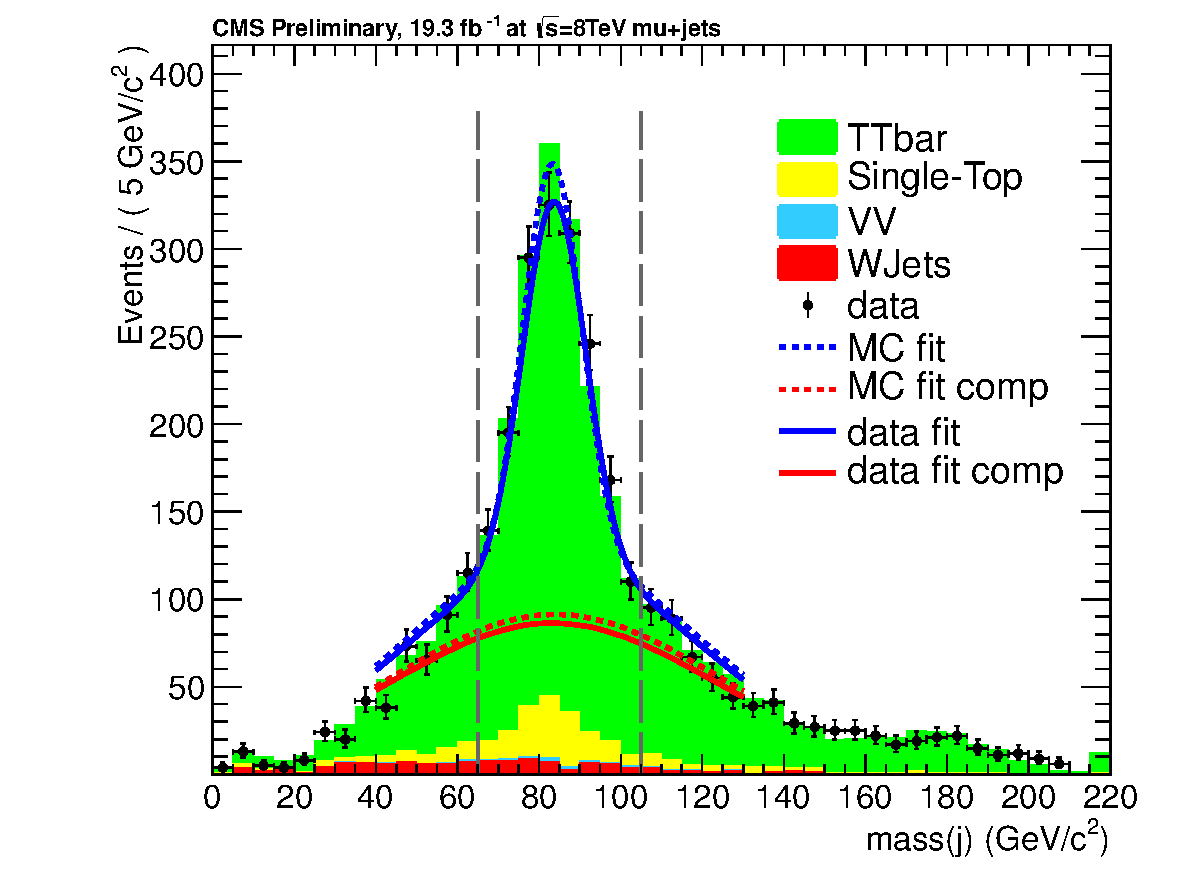
\includegraphics[width=0.45\textwidth]{figs/topwjes/control_medium_mu_with_tau2tau1.pdf}\\
\caption{Pruned jet mass distribution in the $t\bar{t}$ control sample before (left) and after (right) applying $\tau_2/\tau_1<0.55$ cut.}
\label{fig:ttbarControl_nocut}
\end{figure}
%%%%%%%%%%%%%%%%%%%%%%%%%%%%%

%--------------------------------------------------
\subsection{Lepton selection and trigger efficiency}
\label{sec:LeptonSelectionAndTriggerEfficiency}
%%The lepton trigger and selection is common among several CMS analyses and 
%%we benefit from common studies based on tag-and-probe techniques. 
%%
Systematic uncertainties in the trigger efficiencies in
Section~\ref{sec:Eff} are of the order of 1\%. Systematic
uncertainties in the lepton reconstruction and identification
efficiency scale factors are of the order of 2\%. These uncertainties
are accounted for in the final systematics that are input to the
cross-section uncertainty calculation.
%--------------------------------------------------
\subsection{MET uncertainty}
MET directly affects our signal acceptance. 
The uncertainty prescription is discussed in Ref.~\cite{met}.
%https://twiki.cern.ch/twiki/bin/viewauth/CMS/MissingETUncertaintyPrescription
In addition, the MET distribution in the data is $\simeq$3\% wider 
than the MC, and placing a hard MET$>30.0$ cut creates an uncertainty. 
We estimate it by smearing the MET for each event by a Gaussian with 
a $\sigma =0.03*$MET and observing how many events pass the cut. 
Specifically, (Events Passing After Smearing)/(Events Passing Before Smearing) 
=0.998 for both muons and electrons.
%%%%%%%%%%%%%%%%%%%%%%%%%%%%
\subsection{Cross-section of nuisance backgrounds}
The uncertainties in the cross sections of other backgrounds 
like $\ttbar$,  single top, QCD multi-jets, and Z+jets processes 
are already propagated by letting their normalization (i.e., yield) 
float in the fit within a constraint.

%%%%%%%%%%%%%%%%%%%%%%%%%%%%%
\subsection{Theory uncertainty in acceptance}
The theory uncertainty on the signal acceptance due to variations in the parton distribution functions and the
value of $\alpha_{s}$ is obtained by following the {\sc pdf4lhc} prescription ~\cite{Botje:2011sn}.
Using \textsc{CT10}~\cite{ct10}, \textsc{MSTW08}~\cite{Martin:2009iq}, and \textsc{NNPDF}~\cite{nnpdf} sets, the uncertainties are estimated to be 2.3\% 
for $q\bar{q} \to WW$ and and 0.8\% for $gg \to WW$ by the leptonic $WW$ group (SMP-12-024).
Likewise, the impact of higher-order corrections is estimated by varying the QCD renormalisation
($\mu_R$) and factorization ($\mu_F$) scales up and down by a factor of two using the \textsc{mcfm} program~\cite{MCFMarticle} and found to be 1.5\%. 
The overall theory uncertainty is below 3\%, consistent with our studies at 7~TeV (AN-12-224).



%For the 7TeV analysis we compute theory uncertainty in acceptance for muon ``no b-tag'' selection 
%using MCFM: $\pt^{\text{jet}}>35$~GeV, $|\eta^{\text{jet}}|<2.4$, 
%$\pt^{\text{lepton}}>325$~GeV, $|\eta^{\text{lepton}}|<2.1$, 
%$\met > 30$~GeV, W $m_T > 30$~GeV, $\Delta{R}$ (lepton, jet) $>0.3$, 
%no additional lepton. 
%We use CTEQ6.6m as the default PDF and the quantity $\mu_0 = \sqrt{M_W^2 + p_{T, W}^2}$ as  
%the default factorization/renormalization scale.
%For systematic studies 
%we vary the choices of PDF and the factorization/renormalization 
%scale. The details are shown in Table~\ref{tab:theorysyst}. 
%The overall theory 
%uncertainty is below 3\%.
% %%%%%%%%%%%%%%%%%%%%%%%%%%%
% \begin{table}[h!]
%   \begin{center}
%   \begin{tabular}{l|c}
%  \hline
%  \hline
%  Source of uncertainty & Relative variation in acceptance value \\
%  \hline                                  
%  PDF: CT10                             & $1.4\%$ \\
%  PDF: CTEQ61M                          & $-0.7\%$ \\
%  PDF: MSTW8NL                          & $0.4\%$ \\
%  PDF: MSTW8NN                          & $0.1\%$ \\
%  PDF: MSTW8LO                          & $-1.3\%$ \\
%  Scale: $2~\mu_0$                      & $-0.01\%$ \\
%  Scale: $0.5~\mu_0$                    & $0.8\%$ \\
%  Scale: $\sqrt{M_W^2 + p_{T, jet1}^2}$ & $-0.3\%$ \\
%  Scale: $H_T$                          & $0.1\%$ \\
%  \hline
%  \hline
%   \end{tabular}
%   \end{center}
%   \caption{Theory uncertainty in acceptance. The central value for 
%   acceptance $\times$ branching fraction is $(1.279 \pm 0.019) \times 10^{-2}$.} 
%   \label{tab:theorysyst}
% \end{table}
% %%%%%%%%%%%%%%%%%%%%%%%%%
%%%%%%%%%%%%%%%%%%%%%%%%%%%%
\subsection{Uncertainty in jet veto efficiency}
Since we use events with exactly two jets, we reject signal events 
which have extra jet(s) from ISR or FSR. Our acceptance computation 
takes this inefficiency into account. However, there is a 
systematic uncertainty associated with the modeling of 
ISR/FSR in our simulation. The effect has been studied by the WW group and is expected to be less than 5\% (SMP-12-024).

%For the 7TeV analysis, to estimate this systematics we 
%compare the efficiency of our jet veto at generator-level 
%(i.e., using ``GenJets'') in the Pythia WW, Pythia WZ, and 
%privately produced MadGraph WW samples. All three simulations 
%use LO matrix element calculation, parton showering from 
%Pythia, and identical choices of factorization/renormalization
%scales and PDFs. However, the soft gluon radiation probability 
%is different in each sample.  
%Table~\ref{tab:jetvetoeff} lists the jet-veto efficiency 
%in each of the three samples. We take the maximum 
%difference in efficiency as a systematic uncertainty.
%This systematic is within 2\%.
%%%%%%%%%%%%%%%%%%%%%%%%%%%
% \begin{table}[h!]
%   \begin{center}
%   \begin{tabular}{l|c}
%  \hline
%  \hline
%  Sample & jet-veto efficiency \\
%  \hline                                  
%  WW Pythia                             & $88.72\%$ \\
%  WZ Pythia                             & $87.48\%$ \\
%  WW MadGraph                           & $89.57\%$ \\
%  \hline
%  \hline
%   \end{tabular}
%   \end{center}
%   \caption{Jet-veto efficiency in various diboson simulations.} 
%   \label{tab:jetvetoeff}
% \end{table}
%%%%%%%%%%%%%%%%%%%%%%%%%%
%%%%%%%%%%%%%%%%%%%%%%%%%%%%
\subsection{Luminosity uncertainty}
\label{sec:LumiUncertainty}
The latest recommendation for the uncertainty on LHC luminosity is 2.6$\%$~\cite{lumiPAS}.
We propagate this uncertainty to the expected yield of the signal and from there to the
calculated cross-section.
%%%%%%%%%%%%%%%%%%%%%%%%%%%%
%%%%%%%%%%%%%%%%%%%%%%%%%
 \begin{table}[h!]
   \begin{center}
   \begin{tabular}{l|c}
  \hline
  \hline
  Source of uncertainty & Magnitude \\
  \hline                                  
  Luminosity                             & 2.6\%$ \\
  \hline 
  Jet energy scale, resolution, and \MET & $<1\%$ \\
  Theory acceptances (PDF)               & $<3\%$ \\
  ISR/FSR acceptances                    & $<5\%$ \\
  Lepton trigger eff.                    & $1\%$ \\
  Lepton selection eff.                  & $2\%$ \\
  Pile-up                                & $<1\%$ \\
  b-tag veto                             & $<1\%$  \\
  \hline 
  total (without Luminosity)             & $<6.5\%$  \\
  \hline
  \hline
   \end{tabular}
   \end{center}
   \caption{Sources of signal systematics considered in the analysis, with the corresponding magnitude.} 
   \label{tab:signalSyst}
 \end{table}
%%%%%%%%%%%%%%%%%%%%%%%%%
